% ===========================================================================
% Supplementary Information.
%
% NOTHING IS DELETED FROM THIS MANUSCRIPT -- material that does not fit the
% main text's budget is MOVED here, intact. Each note is a self-contained
% argument with its own heading, cited by name from the main text.
%
% Numbering restarts and is independent of the main text (Supplementary
% Note 1, Supplementary Fig. 1, Supplementary Table 1, ...).
% ===========================================================================
\clearpage
\setcounter{figure}{0}\renewcommand{\thefigure}{S\arabic{figure}}
\setcounter{table}{0}\renewcommand{\thetable}{S\arabic{table}}
\setcounter{equation}{0}\renewcommand{\theequation}{S\arabic{equation}}
\setcounter{section}{0}
\renewcommand{\thesection}{Supplementary Note \arabic{section}}

\section*{Supplementary Information}

% Each relocated block goes below as its own \subsection*{Supplementary Note N: ...}
% with a one-line statement of what it contains and which main-text sentence
% points at it.

\subsection*{Supplementary Note 1: The fixed-cost headroom argument}
\label{sec:supp-note-1}

Relocated from the Introduction, where it followed the statement that the $\Theta(m)$ bitmap
kernel pays the same fixed cost regardless of skew, spending most of that cost combining zeros
against zeros (main text).

That waste is not an anecdote about one kind of data; it is a property of the fixed cost itself,
and its size can be settled before any kernel is written. Every alternative encoding of the same
set --- a sorted array of its elements, a list of its maximal runs, a fill-compressed word stream,
or any of these applied to its complement --- is exact and interconvertible with the bitmap, and
each is sized by the set rather than by the universe. The cheapest of them is smaller than the
bitmap by a factor that grows without bound as either operand moves away from density one half, so
a flat cost provably leaves headroom at every density but the middle of the range, for a single
operation as much as for a workload of them. Assuming nothing about the data beyond its density
gives a floor on that headroom rather than an estimate of it: independently placed elements are the
worst case for every encoding whose cost depends on how a set is arranged, so real structure moves
those encodings further below the bitmap and never above it. What this paper optimizes is
therefore not how fast a kernel runs but how much of the computation is never entered. The same
analysis says where that is not possible. Around density one half no encoding is smaller than the
bitmap and nothing can be skipped; there the fixed-cost kernel is the right one, and the return
comes from executing it as fast as the hardware allows --- which is what two decades of vectorized
\texttt{AND}-and-popcount engineering already deliver \cite{mula2018popcount}. Avoid the work where
it can be avoided, accelerate it where it cannot: this paper contributes the first axis, and a
cheap way of knowing which of the two applies.

\subsection*{Supplementary Note 2: Narrowing the query}
\label{sec:supp-note-2}

Relocated from the Introduction, where it followed the statement of Roaring's fixed, per-chunk
granularity (main text).

All of that leaves the caller's question untouched, and a caller willing to narrow it can be given
more. If only pairs above a similarity threshold are wanted, or only operands inside a band of set
sizes, then the two cardinalities alone cap the similarity a pair can reach, so most pairs are
discarded before either operand is read \cite{swamidass2007bounds,bayardo2007allpairs} --- knowing
what is being looked for is itself a way of not doing work, and it is the cheapest one available.

\subsection*{Supplementary Note 3: Thresholded-mode filtering --- the size bound and prefix
filtering}
\label{sec:supp-note-3}

Full derivation for the opt-in thresholded mode named third in the mechanism ladder that opens
Results, and stated with its hypotheses in Methods, ``What makes work avoidable''
(Eq.~\eqref{eq:sizebound}--\eqref{eq:shortfall}): only pairs whose Jaccard similarity or intersection
size clears a threshold are reported. Two mechanisms serve that mode, and the cheaper of them touches
no data whatsoever. Because $|A \cap B| \le \min(a,b)$ while $|A \cup B| \ge \max(a,b)$, a pair's
similarity is capped by the ratio of its two sizes, $J(A,B) \le \min(a,b)/\max(a,b)$, so a pair whose
sizes differ by more than a factor $1/t$ cannot reach the threshold and is discarded from two
integers, before either operand is read. An absolute threshold behaves the same way: $|A \cap B| \ge
\tau$ requires only $\min(a,b) \ge \tau$. Restricting the \emph{inputs} to a band of sizes --- ignoring
the extremely rare, or keeping only those --- is that same comparison applied before a pair is formed
rather than after. The bound is the Swamidass--Baldi pruning result \cite{swamidass2007bounds}
together with the size filter of the similarity-join literature \cite{bayardo2007allpairs,xiao2008ppjoin};
what is reported here is not the bound but where it sits relative to the rest and how it composes with
them.

How much it removes is fixed by one property of the corpus, and that property is what makes it worth
separating from the mechanisms above. Under the $1/i$ cardinality spectrum this paper benchmarks ---
cardinalities log-uniform on $[1,K]$, which is the density $\Pr(a) \propto 1/a$ exactly, so this is the
mandated spectrum and not a stand-in for it --- the fraction of pairs that can possibly qualify is
$1 - (1 - \ln(1/t)/\ln K)^{2}$ (Methods, Eq.~\eqref{eq:survive}), which agrees with a $10^{5}$-sample
simulation to three decimals. At $K = 10^{4}$ that leaves $14.5\%$ of pairs at $t = \tfrac12$, $4.8\%$
at $t = 0.8$, $2.3\%$ at $t = 0.9$ and $1.1\%$ at $t = 0.95$, so examining every pair does $6.9\times$
to $90.0\times$ the work of examining only the survivors. \textbf{The expression falls as $K$ rises:
the wider the spread of set sizes, the more pairs are ruled out by the ratio alone.} That is the
reverse of the dependence every other mechanism in this paper has. The null models of
Fig.~\ref{fig:density-sweep} are all stated at a \emph{fixed} density and bound what a mechanism is
worth against within-row arrangement; the size bound is the only one whose value is a function of the
\emph{dispersion of cardinalities across the corpus}, and it strengthens monotonically as that
dispersion widens --- $2.3\%$ surviving at $K = 10^{4}$ against $1.1\%$ at $K = 10^{8}$, both at $t =
0.9$. The two axes are different and not in competition. One limit is worth stating with it: the
favourable scaling belongs to this spectrum rather than to skew in general, and under a heavier tail in
which \emph{ranked} sizes scale as $1/i$ the surviving fraction is exactly $1 - t$ whatever $K$ is
(Methods, ``What makes work avoidable'').

It does not, however, multiply with the mechanisms below it, and the reason refines the composition
rule this section has otherwise used. Deciding whether a pair exists at all is the coarsest
granularity in the paper, so the rule as stated predicts a clean product with anything acting inside a
pair. The product is not achieved. The survivors of the size test are the pairs with $a \approx b$, and
representation choice, a zone map and the prefix filter are each cheapest precisely when the two sizes
are \emph{dissimilar} --- so the test passes on the pairs the rest serve worst, and the composed cost
exceeds the product of the two savings by the factor that conditioning raises a survivor's mean cost,
$\ln K / 2$ in the limit of a high threshold (Methods, Eq.~\eqref{eq:shortfall}). At $K = 10^{4}$, $t =
0.9$ and $m = 10^{6}$ the size bound leaves $2.76\%$ of pairs and representation choice costs $1.51\%$
of a bitmap, so a product would predict $0.042\%$ where the composition costs $0.151\%$. Replaying the
same composition with the size test decorrelated from cardinality, at an identical survival rate,
restores the product to within $0.6\%$, which identifies the shared statistic rather than the shared
granularity as the cause. The composition remains firmly worth taking --- it costs $10.0\%$ of the
better of the two mechanisms alone, and a bitmap pass over every pair does $660\times$ its work --- so
what this refutes is the product, not the composition. \textbf{Mechanisms compose multiplicatively when
they act on different waste \emph{and} read different operand statistics; acting at different
granularities is necessary and not sufficient.} These are analytic values over the model above, and
like the rest of this note they count work rather than time.

The thresholded mode changes the contract rather than the kernel: only pairs above a similarity
threshold are reported, and the second mechanism that exploits that is prefix filtering rather than any
representation choice. It admits the same analysis, and it reduces further than the others do. Because
a qualifying pair must share an element between its prefixes, the entire behaviour of the filter is
governed by one dimensionless quantity --- the expected number of shared prefix elements per pair, $y =
p^{2}/m$ --- and the fraction of pairs surviving is $1 - e^{-y}$ regardless of density, threshold or
universe size separately (Supplementary Fig.~\ref{fig:prefix}). Below $y = 1$ pruning improves quadratically
as
prefixes shorten; above it prefixes collide by default and the index earns nothing. \spec{That single
variable is what a gate for this mode should test, and it is cheap to compute from the metadata already
held.}

\begin{figure}[!t]
\centering
\footnotesize
\textbf{a}\par\vspace{0.4mm}
% Prefix-filtering schematic (was Fig. 1e)
% Extracted from the former Fig. 1; rendered as a panel of its own figure.
\centering
% ===========================================================================
% Figure 1 — overview. Body only; \input inside a figure environment.
% House idiom follows the scaffold paper's fig:planes: minipage panels with
% bold letter labels, \resizebox per panel, and the two-saturation convention
% (strong fill = the lanes the panel is about, faint same-hue fill = context).
%
% Requires simdgrid.sty and the repr* colours from storm.tex.
% ===========================================================================

% Focus / context saturations, one pair per representation.
\colorlet{focB}{reprB!45}\colorlet{ctxB}{reprB!12}
\colorlet{focS}{reprS!55}\colorlet{ctxS}{reprS!14}
\colorlet{focR}{reprR!55}\colorlet{ctxR}{reprR!14}
\colorlet{focW}{reprW!55}\colorlet{ctxW}{reprW!14}
\colorlet{focC}{reprC!65}\colorlet{ctxC}{reprC!18}
\colorlet{zone}{black!18}

\tikzset{
  gridcell/.style={draw=black!55, line width=0.4pt, minimum width=16.5mm,
                   minimum height=6.6mm, inner sep=1pt, font=\scriptsize,
                   anchor=center},
  hdr/.style={font=\scriptsize\bfseries},
  flowbox/.style={draw=black!60, rounded corners=1.2pt, align=left,
                  font=\scriptsize, inner sep=3.2pt},
  flowarrow/.style={-{Latex[length=1.8mm]}, draw=black!65, line width=0.5pt},
}

% ------------------------------------------------------------------ panel e
% Prefix filtering: a candidate-pruning rule from the similarity-join
% literature, used only in the opt-in thresholded mode.
\centering
\resizebox{.23\linewidth}{!}{%
\begin{tikzpicture}[x=1mm,y=1mm]
  \tikzset{sm/.style={draw=black!55, line width=0.35pt},
           tiny lbl/.style={font=\scriptsize, text=black!70}}
  % Type size: cell values were \tiny against \scriptsize row labels, and the
  % whole picture was then scaled up ~1.9x, so the labels rendered about 15 pt
  % -- larger than the body text and roughly four times the neighbouring
  % matplotlib panels. Every glyph is \scriptsize now and the picture is set
  % near its natural size, so it renders at ~8 pt like everything around it.
  % Encoding, not prose: prefix = saturated, tail = near-white, the shared
  % element = accent. The verdict is a glyph. The caption narrates.
  %
  % Prefix-versus-tail is a pure LUMINANCE axis (mid ink against near-white),
  % so it survives greyscale on its own and costs no hue. It used to be drawn
  % in S's blue and the shared element in R's green, which spent two
  % representation hues on things that are not representations. The shared
  % element is what makes the pair survive to exact verification, so it now
  % takes the same reserved "work" accent used everywhere else in the paper,
  % and the discarded pair takes the "work avoided" accent.
  \definecolor{workc}{HTML}{EE6677}
  \definecolor{avoidc}{HTML}{66CCEE}
  \colorlet{pfx}{black!26}\colorlet{tail}{black!5}\colorlet{hit}{workc}
  \newcommand{\prefrow}[5]{% #1 y  #2 label  #3 prefix  #4 tail  #5 hit index (-1 none)
    \node[font=\scriptsize\bfseries, anchor=east] at (-1.4,#1+2.1) {#2};
    \foreach \v [count=\k from 0] in {#3}{
      \ifnum\k=#5 \def\f{hit}\else\def\f{pfx}\fi
      \draw[sm, fill=\f] (\k*5,#1) rectangle ++(5,4.2);
      \node[font=\scriptsize\bfseries] at (\k*5+2.5,#1+2.1) {\v};}
    \foreach \v [count=\k from 0] in {#4}{
      \draw[sm, draw=black!35, fill=tail] (\k*5+10,#1) rectangle ++(5,4.2);
      \node[font=\scriptsize, text=black!45] at (\k*5+12.5,#1+2.1) {\v};}}
  % verdict glyphs, drawn rather than set as text
  \newcommand{\vdiscard}[2]{\draw[line width=1.1pt, draw=avoidc!55!black]
      (#1-1.7,#2-1.7) -- (#1+1.7,#2+1.7) (#1-1.7,#2+1.7) -- (#1+1.7,#2-1.7);}
  \newcommand{\vkeep}[2]{\draw[line width=1.2pt, draw=workc!65!black,
      line cap=round,
      line join=round] (#1-1.9,#2+0.1) -- (#1-0.5,#2-1.5) -- (#1+2.0,#2+1.9);}

  \draw[-{Latex[length=1.3mm]}, draw=black!45, line width=0.4pt] (0,10.4) -- (10,10.4);
  \node[font=\scriptsize, text=black!55, anchor=west] at (10.8,10.4) {rarest first};
  \prefrow{0}{$A$}{17,4}{23,8,31}{-1}
  \prefrow{-6}{$B$}{12,23}{8,31,5}{-1}
  \draw[decorate, decoration={brace, amplitude=2.2pt}, draw=black!55]
    (0,4.7) -- (10,4.7) node[midway, above=1.8pt, font=\scriptsize, text=black!65] {prefix};
  \vdiscard{31}{-3}

  \begin{scope}[shift={(0,-11.5)}]
    \prefrow{0}{$A$}{17,4}{23,8,31}{1}
    \prefrow{-6}{$C$}{4,12}{8,31,5}{0}
    \vkeep{31}{-3}
  \end{scope}
\end{tikzpicture}}


\vspace{2mm}
\par\vspace{0.6mm}
% Generated at exactly \textwidth and included unscaled. At the previous .50
% every label on this figure rendered below 4 pt.
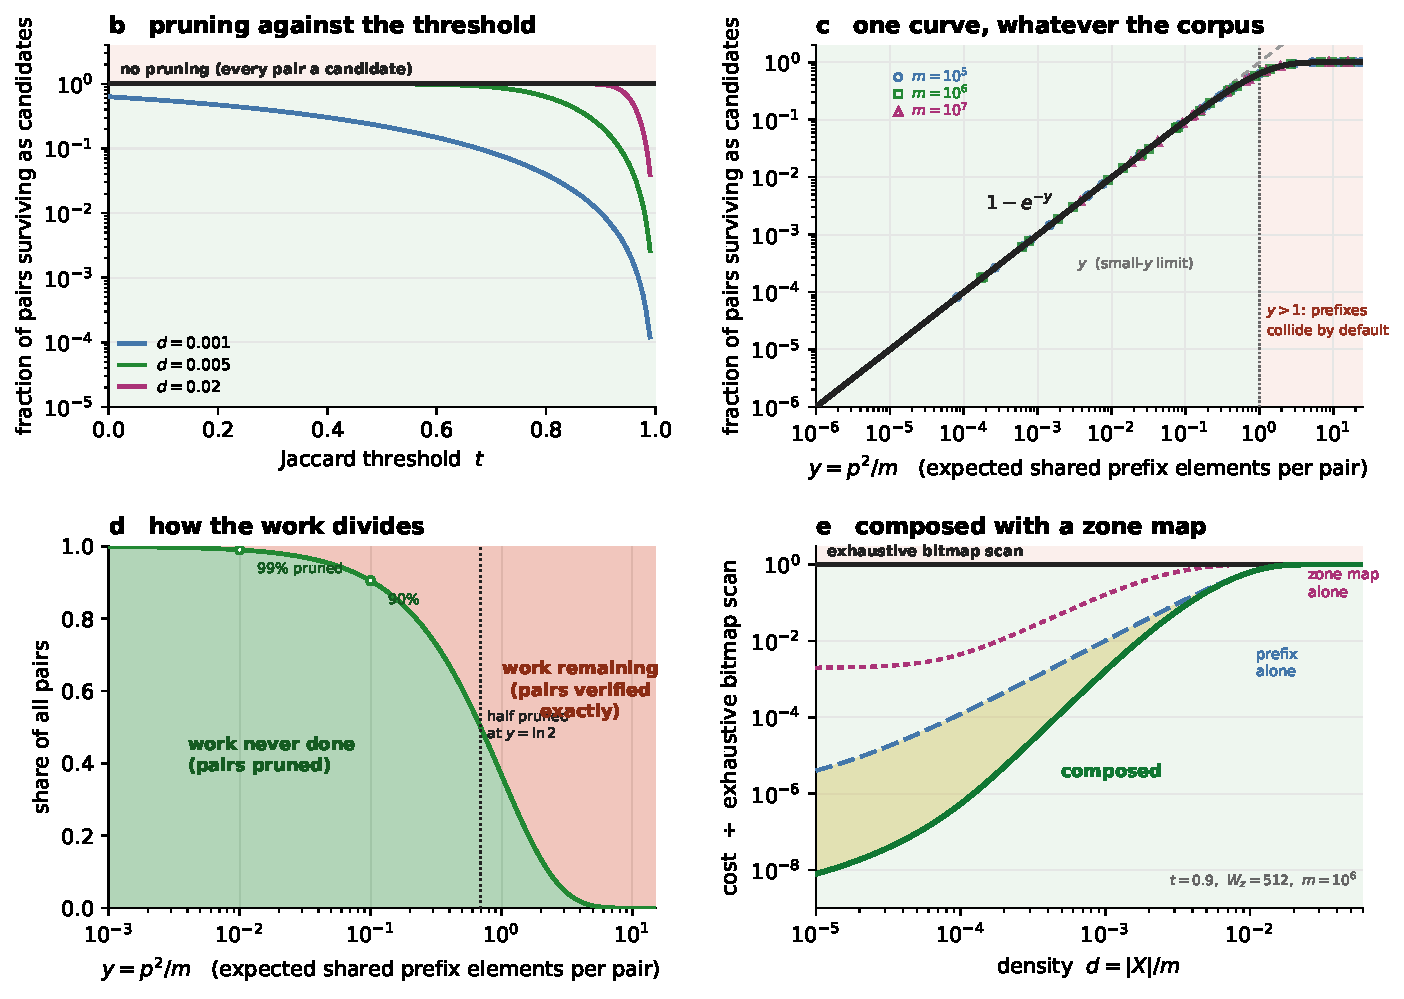
\includegraphics[width=\linewidth]{figures/fig3_prefix}
\caption{\textbf{Prefix filtering, analysed on the same terms --- and reducible to a single
variable.} Prefix filtering serves the opt-in thresholded mode, in which only pairs of Jaccard
similarity at least $t$ are reported. With elements in a global order and prefix length
$p(X) = |X| - \lceil t|X| \rceil + 1$, any qualifying pair must share an element between its
prefixes, so indexing prefixes alone answers the thresholded question exactly --- and unlike the
mechanisms of Fig.~\ref{fig:density-sweep}c--d it is candidate \emph{generation}: the quadratic pair
set is never enumerated. Reading key as in Fig.~\ref{fig:density-sweep}; an ordered series takes a
sequential ramp with its own marker or dash pattern.
\textbf{a}, How the rule works. Elements are laid out rarest first, hence the non-monotonic labels,
and each set's prefix (saturated) is its rarest $p(X)$ elements. Top: the prefixes share no element,
so the pair is discarded without computing any intersection. Bottom: one element appears in both,
marked in red because it is what commits the pair to exact verification.
\textbf{b}, Fraction of pairs surviving as candidates against the threshold, at universe $10^{6}$.
Prefix length falls as $t$ rises, so the filter that removes almost everything at a high threshold
removes almost nothing at a low one, and denser operands need a higher threshold to prune as hard.
\textbf{c}, All of that collapses onto one curve. For prefixes of length $p$ over a universe of $m$
the expected number of shared prefix elements per pair is $y = p^{2}/m$, and the surviving fraction
is exactly $1 - e^{-y}$ for scattered operands; markers are $(d,t,m)$ combinations drawn at random,
and lie on the curve by construction rather than by fit. For $y \ll 1$ the surviving fraction is $y$
itself; for $y > 1$ prefixes collide by default and the index is pure overhead. So $y$ --- not $t$,
and not density --- is what a selector should test.
\textbf{d}, The same as a division of labour: pairs never examined against pairs surviving to exact
verification. The two are equal at $y = \ln 2$.
\textbf{e}, Prefix filtering composed with a zone map. Unlike the two mechanisms of
Fig.~\ref{fig:density-sweep}c these \emph{do} compose --- their savings multiply, to within \nm{a
factor of 1.25 at the sparsest end, exactly elsewhere; analytic} --- because they act on different
waste and read different statistics. At $d = 10^{-3}$, $t = 0.9$ and $W_z = 512$ the composition
costs \nm{$\approx 0.17\%$, analytic} of an exhaustive bitmap scan, against $1.0\%$ for prefix
filtering alone and $16\%$ for a zone map alone.
Analytic throughout; no measured data, and like Fig.~\ref{fig:density-sweep} it models work rather
than time. \spec{Real corpora deviate in the same direction as elsewhere: frequency-ordered prefixes
concentrate rare elements, so real prefixes collide less than scattered ones of the same length and
the true curve lies below this one.}}
\label{fig:prefix}
\end{figure}

\subsection*{Supplementary Note 4: Derivation of the zone-map cost model and its crossings}
\label{sec:supp-note-4}

Relocated from Results, ``The cost of intersection is U-shaped in density,'' which points here for
the full derivation behind Fig.~\ref{fig:density-sweep}b--d: the null-model floor, the four counting
properties of a zone map (why it has a floor, why the leverage is large, why the advantage is flat
then erodes quadratically, and why it can be a liability), the crossing densities, and the
work-versus-time distinction.

Every panel of Fig.~\ref{fig:density-sweep} is the same argument applied to a different mechanism,
and it is worth stating that argument once. Each mechanism --- choosing a representation, consulting
a zone map, composing the two, and in the thresholded mode the prefix filter of
Supplementary Fig.~\ref{fig:prefix}
--- is a bet that the data deviates from randomness, and each comes with a closed-form null model
saying what the bet is worth if it does not. Fixing the density and placing elements independently is
the most pessimistic assumption available about \emph{arrangement}, and it is pessimistic in the same
direction for all of them: independent placement maximises the number of maximal runs a set has,
maximises the fraction of bins it occupies, and maximises the chance that two prefixes collide.
\textbf{The null model is therefore a floor and not a prediction.} Real structure can only move each
mechanism further into profit, and the size of that movement is exactly what the mechanism converts
into speed.

Two things a fixed design cannot do follow immediately, and they are the reason the selector is built
the way it is. A representation committed to at ingest cannot exploit the deviation, because it
commits before the deviation is knowable. A selector reading density alone cannot exploit it either,
because density is the very statistic the null model is built from: at a fixed density $d$ with
$k = dm$ elements the expected number of maximal runs is $k(m-k+1)/m$, but the actual number ranges
over every integer from one to $\min(k,\,m-k+1)$, so no single function of $d$ can track it. The
deviation is also \emph{one-sided} --- a real row can be arbitrarily cheaper than a random row of the
same density and at most about twice as expensive (Methods, ``What makes work avoidable'') --- which
is what makes it a resource
rather than a source of variance. Both readings point the same way: the statistic a selector consults
has to see arrangement, or be a direct measurement of the kernels themselves.

Four properties of the summary in Fig.~\ref{fig:density-sweep}b--c follow from counting alone, and
they are worth stating plainly because together they say what a summary can and cannot buy.

\emph{Why there is a floor, and where it is.} A zone map is a bitmap of bitmaps: one bit per bin of
$W_z$ positions, so $m/W_z$ bits against the row's $m$. Reading it therefore costs $1/W_z$ of reading
the row, and no pairing that consults a summary can cost less than reading that summary --- $0.195\%$
of a bitmap at $W_z = 512$. That is the floor, and it is a property of the bin width alone, not of the
data.

\emph{Why the leverage is so large.} The exchange rate is the same $W_z$: one summary bit decides the
fate of $W_z$ data bits, so a bin proved empty returns $W_z$ bits of work for the one bit spent
asking. This is why a coarser bin buys a deeper floor --- and, symmetrically, why it stops paying at a
lower density, since a wider bin is harder to leave empty.

\emph{Why the advantage is flat across the sparse range and then erodes quadratically.} A bin
survives only if \emph{both} operands occupy it, so the surviving fraction goes as the product of the
two occupancies. For clustered operands, where a run longer than a bin occupies exactly a $d$ fraction
of bins, that product is $d^2$, and the cost is $1/W_z + d^2\kappa$ with $\kappa$ the cost of a bin's
contents. The two terms are equal when $d^2\kappa = 1/W_z$; with $\kappa$ the cost of one run in a
bin, $\kappa = w/W_z$, this reduces to $d = 1/\sqrt{w} = 1/8$ --- \textbf{independent of the bin
width}. Below that density the summary term dominates and the advantage is constant; above it the
surviving-bin term dominates and the advantage decays as $d^{2}$. Changing $W_z$ moves the floor but
not the knee.

\emph{Why a summary can be a liability, and exactly when.} The floor cuts both ways, and the reason is
structural rather than a property of any one representation: \textbf{a summary is indexed by the
universe, while every compressed representation is indexed by the data}. The zone map costs $1/W_z$
of a bitmap whatever the operands contain, because its size is set by $m$. The cost of $\rS$, $\rR$
and $\rW$ is set instead by a quantity that shrinks with the set --- cardinality, run count, or
literal-and-fill count --- and each of those falls without limit as the operands sparsify. A fixed
cost and a vanishing one must cross. \textbf{Below that crossing, consulting a summary costs more than
the entire computation it was meant to shorten, and a zone map is worse than not having one.}

Where the crossing falls depends on which representation is being displaced, and one case fixes the
scale. A representation costing one word per element costs $w\,d$ of a bitmap, so it meets the
summary's $1/W_z$ at $d = 1/(wW_z) = 3.1\times10^{-5}$ for $w = 64$ and $W_z = 512$ (Methods,
Eq.~\eqref{eq:dlow}). At $d = 10^{-6}$ that representation costs $6.4\times10^{-5}$ of a bitmap while
the summary alone costs $1.95\times10^{-3}$, so consulting it does $31\times$ the work of simply
enumerating the operands. A run- or fill-based representation crosses at its own density, wherever its
run or word count falls below $m/W_z$, but that a crossing exists at all is generic.

This makes the gating two-sided, and for two unrelated reasons. A summary must be declined when the
operands are \emph{too dense}, because every bin is occupied and it proves nothing; and equally when
they are \emph{too sparse}, because it is then the largest object in the computation. It pays only
between those two bounds. \spec{The same fact appears in the storage measurements as
universe-proportional selector metadata dwarfing the data it describes; the time and space statements
of it are one phenomenon, and a guard on one is a guard on the other.}

The practical reading is that the sparse regime is not a narrow operating point. In the clustered
idealization --- the favourable edge of the band, where a run spans a whole bin --- the advantage is
the same at $d = 10^{-6}$ as at $d = 10^{-2}$: five orders of magnitude of density over which a
fixed-cost kernel does $512\times$ the work of one that consults a summary first. It is only above
$d = 1/8$ that the margin narrows at all, and even at $d \to 1$ a bitmap still does $7.9\times$ the
work.

All of the quantities above are counts of $64$-bit words touched, not times, and the distinction is
load-bearing rather than pedantic. A work model prices a summary that removes nothing at its own size,
$1/W_z$ of a bitmap, and that is a correct statement about words. It is not a statement about runtime:
a filtered scan gives up sequential access and hardware prefetch and pays an indirection and a branch
per bin, and the measured penalty for consulting a summary on operands it cannot help is far larger
than these panels charge --- \nm{worst-case speedup, filter applied unconditionally, which the work
model does not predict} against the $1.002\times$ overhead the work model allows, matching the
always-on-versus-gated contrast reported directly in Results, ``Selection must be hoisted, and
measured rather than modelled'' (Fig.~\ref{fig:selection-cost}c). That divergence is not a defect in
the derivation; it is the reason the gate is decided by measurement rather than by the model, and the
per-bin and per-word constants needed to convert these curves into time are given in Methods.

\subsection*{Supplementary Note 5: What repeats across a batch, and how each mechanism amortises it}
\label{sec:supp-note-5}

Relocated from Results, ``Selection must be hoisted, and measured rather than modelled,'' which points
here for the four quantities that repeat when a batch of pairs is run naively and how each is
amortised instead.

The contract is unchanged and the answer is identical, but batch amortisation requires many
operations rather than one, because what it removes is not work but \emph{repetition}. Four things
repeat when a batch is run naively, and each can be paid for once instead. Row metadata ---
cardinality, run count, occupancy summary --- is part of the representation, built at ingest and
amortised over every operation the set ever participates in rather than over any particular batch;
this is the same assumption Roaring's per-chunk container choice already makes, and it is stated here
once for the whole paper. A selection decision can be hoisted to a tile, so one decision serves a
block of pairs instead of one pair. Probe-and-commit pays to time a handful of operations and reuses
the verdict for the rest. And operand data loaded once can be paired against many, so its memory
traffic is amortised rather than repeated. In each case the same thing happens: the decision and the
metadata are amortised, and only the kernel work stays per operation (Supplementary
Fig.~\ref{fig:batch}b).
This is a regime rather than the setting. It applies wherever there are enough operations to share a
decision --- which is a property of a workload of any size, not an argument that anything must be
computed exhaustively --- and it is the regime in which the selection-cost measurements of the main
text were taken. The single-operation regime is reasoned instead from the cost of a decision read from
$O(1)$ metadata against the size of the operation it governs, and the asymmetry in evidence between
the two is stated here rather than left to be inferred.

Two mechanisms of that regime are drawn together in Supplementary Fig.~\ref{fig:batch}: an overlap
pre-filter that settles most of a pair set from summaries alone, and the way a decision's cost is
governed by the size of the operation it is made about.

\begin{figure}[!t]
\centering
% Column-postings tile pipeline. Body only; input inside a figure environment.
\definecolor{workc}{HTML}{EE6677}
\definecolor{avoidc}{HTML}{66CCEE}
\colorlet{zone}{black!20}

\tikzset{
  postcell/.style={draw=black!55, line width=0.35pt},
  postlabel/.style={font=\scriptsize, text=black!75},
  pipebox/.style={draw=black!60, rounded corners=1.2pt, align=center,
                 font=\scriptsize, inner sep=4pt, minimum height=9mm},
  pipearrow/.style={-{Latex[length=2mm]}, draw=black!65, line width=0.55pt},
}

\textbf{a}\par\vspace{0.6mm}
\resizebox{.96\linewidth}{!}{%
\begin{tikzpicture}[x=1mm,y=1mm]
  % Row-oriented incidence matrix.
  \node[postlabel, font=\scriptsize\bfseries, anchor=west] at (0,5)
    {row occupancy $A_{ib}$};
  \foreach \b in {0,...,3}{
    \node[postlabel] at (14+5*\b,1.7) {$b_{\b}$};}
  \foreach \i in {0,...,5}{
    \node[postlabel, anchor=east] at (10,-3-5*\i) {$X_{\i}$};}
  \foreach \bits [count=\i from 0] in {{1,0,0,1},{1,1,0,0},{0,0,1,0},
                                       {0,1,0,1},{1,0,0,0},{0,0,1,1}}{
    \foreach \bit [count=\b from 0] in \bits {
      \ifnum\bit=1 \def\fillc{zone}\else\def\fillc{white}\fi
      \draw[postcell,fill=\fillc] (11.5+5*\b,-5.5-5*\i) rectangle ++(5,5);}}

  % Explicit transpose into postings.
  \draw[pipearrow] (34,-13) -- (45,-13)
    node[midway,above,postlabel] {transpose};
  \node[postlabel, font=\scriptsize\bfseries, anchor=west] at (46,5)
    {column postings};
  \node[pipebox,fill=zone!65,minimum width=28mm] at (60,0) {$P_0=\{0,1,4\}$};
  \node[pipebox,fill=zone!65,minimum width=28mm] at (60,-10) {$P_1=\{1,3\}$};
  \node[pipebox,fill=zone!65,minimum width=28mm] at (60,-20) {$P_2=\{2,5\}$};
  \node[pipebox,fill=zone!65,minimum width=28mm] at (60,-30) {$P_3=\{0,3,5\}$};

  % Candidate matrix induced by the multi-row postings.
  \draw[pipearrow] (75,-13) -- (87,-13)
    node[midway,above,postlabel,align=center] {OR into\\candidate masks};
  \begin{scope}[shift={(90,0)}]
    \node[postlabel, font=\scriptsize\bfseries, anchor=west] at (0,5)
      {candidate pairs};
    \foreach \j in {0,...,5}{
      \node[postlabel] at (3+5*\j,1.7) {$\j$};}
    \foreach \i in {0,...,4}{
      \node[postlabel,anchor=east] at (-1,-3-5*\i) {$\i$};}
    \foreach \i/\js in {0/{1,3,4,5},1/{3,4},2/{5},3/{5}}{
      \foreach \j in \js {
        \draw[postcell,fill=workc!75] (0.5+5*\j,-5.5-5*\i) rectangle ++(5,5);}}
    \foreach \i/\js in {0/{2},1/{2,5},2/{3,4},3/{4},4/{5}}{
      \foreach \j in \js {
        \draw[postcell,dashed,fill=avoidc!25] (0.5+5*\j,-5.5-5*\i) rectangle ++(5,5);}}
    \node[postlabel,anchor=west] at (2,-33) {candidate};
    \draw[postcell,fill=workc!75] (-4,-35) rectangle ++(5,4);
    \node[postlabel,anchor=west] at (25,-33) {proved empty};
    \draw[postcell,dashed,fill=avoidc!25] (18,-35) rectangle ++(5,4);
  \end{scope}
\end{tikzpicture}}

\vspace{3mm}
\textbf{b}\par\vspace{0.6mm}
\resizebox{.96\linewidth}{!}{%
\begin{tikzpicture}[node distance=8mm and 8mm]
  \node[pipebox,fill=black!8] (gate) {online tile\\gate};
  \node[pipebox,fill=avoidc!18,right=of gate] (range) {sort by minimum\\and reject extents};
  \node[pipebox,fill=zone!55,right=of range] (transpose) {transpose row\\occupancy};
  \node[pipebox,fill=zone!55,right=of transpose] (compact) {retain multi-row\\postings};
  \node[pipebox,fill=workc!22,right=of compact] (resolve) {resolve unique\\candidate masks};
  \node[pipebox,fill=reprS!18,right=of resolve] (verify) {selected exact\\row cell};
  \draw[pipearrow] (gate) -- node[above,postlabel] {postings route} (range);
  \draw[pipearrow] (range) -- (transpose);
  \draw[pipearrow] (transpose) -- (compact);
  \draw[pipearrow] (compact) -- (resolve);
  \draw[pipearrow] (resolve) -- (verify);
  \node[pipebox,fill=reprB!10,below=10mm of transpose] (row) {row-pairing tournament\\for direct-route tiles};
  \draw[pipearrow] (gate.south) |- node[pos=.25,left,postlabel] {direct route} (row.west);
  \draw[pipearrow] (row.east) -| (verify.south);
\end{tikzpicture}}

\caption{\textbf{The batch regime: rejecting pairs wholesale, and paying for a decision once.}
Both mechanisms here need many operations rather than one, and what they remove is repetition.
\textbf{a}, An overlap pre-filter across a set of operands. The same occupancy idea as a zone map
(Fig.~\ref{fig:density-sweep}a) but at a coarser, chosen width and computed once per set, then
ANDed pairwise: shaded pair cells may overlap and are passed to a kernel, dashed cells are provably
disjoint and are answered without touching data. One pass over the summaries settles most of the
pair matrix. Note the distinction from prefix filtering (Supplementary Fig.~\ref{fig:prefix}), which
is candidate \emph{generation} and never enumerates the pair set at all.
\textbf{b}, Why the cost of a decision depends on what it governs. Each bar spends left-to-right
through one unit of useful work; the dashed rule marks that work with neither a decision nor a
filter. \emph{Deciding}: a single operation absorbs the decision easily, since it is read from
$O(1)$ metadata and the operation it governs is large; the same decision repeated for every
operation of a batch is a large fraction of the total, because each operation there is small; and
hoisting it to a tile --- deciding once, then committing --- restores the single-operation picture.
\emph{Filtering}: where bins are mostly empty a summary converts most of the work into skipped work;
where every bin is occupied it finds nothing to skip and its cost carries the bar past the rule.
The cost of deciding therefore scales inversely with how large the operation being decided about is,
which is why the two regimes need different policies and why every mechanism is gated rather than
always on. Schematic; no measured data.}
\label{fig:batch}
\end{figure}

\subsection*{Supplementary Note 6: Corpus provenance and inventory}
\label{sec:supp-note-6}

Supplementary Table~\ref{tab:corpus-inventory} gives full provenance and per-corpus statistics for
every corpus referenced anywhere in this paper, including the corpora scored only against an
all-bitmap baseline and never against CRoaring, which Table~\ref{tab:corpora} summarises in a single
row. It also records, for the two genomic corpora, which axis is treated as the universe under each
storage layout --- the distinction the main text draws in Results, ``Where the method does not
pay.''

% longtable is NOT a float and creates no group, so a bare \scriptsize here
% leaks into every following section. Keep it inside an explicit group.
% Start on a fresh page: the table is a full page of body, so letting it begin
% at the foot of the previous one emits an orphaned "(continued)" head with no
% rows under it.
\clearpage
\begingroup
\scriptsize
\setlength{\tabcolsep}{2.2pt}
% The document-wide \arraystretch{1.20} pushed this table one row past a full
% page, stranding that row behind two unrelated tables. Tightened so the whole
% inventory sits on one page.
\renewcommand\arraystretch{1.0}
% Corpus names are identifiers, so \seqsplit breaking them after one character
% is worse than a wrapped prose note. Width moved from the notes column to the
% name column; the total is unchanged, so the table cannot overflow.
\begin{longtable}{@{}p{3.7cm} l r r r r p{3.5cm}@{}}
\caption{\textbf{Corpora, provenance and statistics.} Every corpus referenced anywhere in this paper,
in four provenance groups used to assemble the benchmark set: \textbf{G1}, the twelve
\texttt{real-roaring-datasets} files CRoaring's own harness runs by default
\cite{chambi2016roaring,lemire2018roaring}; \textbf{G2}, five SNAP social/web graphs (Stanford Large
Network Dataset Collection) scored by neighbourhood-intersection density; \textbf{G3}, two genomic
corpora present for scoping rather than for the headline, included so a reader can judge whether the
benchmark set was chosen favourably; \textbf{G4}, KONECT graphs, UShER SARS-CoV-2, gnomAD and the
\texttt{msprime} coalescent-simulation series, added after the original survey. Density and mean
$|X_i|$ are corpus properties from the data loaders, not timing results. For the two G3 corpora,
\emph{universe} and \emph{rows} swap roles between layouts: \texttt{chr20.bin} is variant-major
(universe = 5{,}008 haplotypes, one row per variant site); \texttt{chr20\_hap.bin} is haplotype-major
(universe $\approx$ 1{,}048{,}576 sites, one row per haplotype) --- the layout dependence discussed in
the main text (Results, ``Where the method does not pay''). ---, not reported by the source.
\draftnote{All values provisional, pending the final measurement campaign.}}
\label{tab:corpus-inventory}\\
\toprule
Corpus & Group & Rows/sets & Universe $m$ & Mean $|X_i|$ & Density & Origin / notes \\
\midrule
\endfirsthead
\multicolumn{7}{l}{\textit{Table~\ref{tab:corpus-inventory} (continued)}} \\
\toprule
Corpus & Group & Rows/sets & Universe $m$ & Mean $|X_i|$ & Density & Origin / notes \\
\midrule
\endhead
\midrule \multicolumn{7}{r}{\textit{continued on next page}} \\
\endfoot
\bottomrule
\endlastfoot
\texttt{\seqsplit{census1881}} & G1 & \prov{200} & \prov{4{,}277{,}806} & \prov{5{,}019} & \prov{1.2e-3} & 1881 Canadian census, categorical attributes \\
\texttt{\seqsplit{census1881\_srt}} & G1 & \prov{200} & \prov{4{,}277{,}735} & \prov{3{,}404} & \prov{8.0e-4} & as above, rows sorted \\
\texttt{\seqsplit{census-income}} & G1 & \prov{200} & \prov{199{,}523} & \prov{34{,}610} & \prov{1.7e-1} & US census income (UCI ``Adult''-family), attributes \\
\texttt{\seqsplit{census-income\_srt}} & G1 & \prov{200} & \prov{199{,}523} & \prov{30{,}464} & \prov{1.5e-1} & as above, rows sorted \\
\texttt{\seqsplit{weather\_sept\_85}} & G1 & \prov{200} & \prov{1{,}015{,}367} & \prov{64{,}353} & \prov{6.3e-2} & September 1985 weather observations, binned attributes \\
\texttt{\seqsplit{weather\_sept\_85\_srt}} & G1 & \prov{200} & \prov{1{,}015{,}367} & \prov{80{,}540} & \prov{7.9e-2} & as above, rows sorted \\
\texttt{\seqsplit{wikileaks-noquotes}} & G1 & \prov{200} & \prov{1{,}353{,}179} & \prov{1{,}377} & \prov{1.0e-3} & WikiLeaks cable corpus, term/attribute postings \\
\texttt{\seqsplit{wikileaks-noquotes\_srt}} & G1 & \prov{200} & \prov{1{,}353{,}133} & \prov{1{,}440} & \prov{1.1e-3} & as above, rows sorted \\
\texttt{\seqsplit{uscensus2000}} & G1 & \prov{200} & \prov{36{,}974{,}578} & \prov{30} & \prov{8.1e-7} & US Census 2000; \textbf{sparsest and largest-universe G1 corpus} \\
\texttt{\seqsplit{dimension\_003}} & G1 & \prov{15{,}482} & \prov{3{,}866{,}847} & \prov{91} & \prov{2.4e-5} & Druid-derived dimension column \\
\texttt{\seqsplit{dimension\_008}} & G1 & \prov{5{,}240} & \prov{3{,}866{,}845} & \prov{347} & \prov{9.0e-5} & Druid-derived dimension column \\
\texttt{\seqsplit{dimension\_033}} & G1 & \prov{173} & \prov{3{,}866{,}847} & \prov{22{,}352} & \prov{5.8e-3} & Druid-derived dimension column \\
\addlinespace
\texttt{\seqsplit{as-skitter}} & G2 & \prov{1{,}696{,}415} & \prov{1{,}696{,}415} & \nm{n} & \prov{9.1e-6} & CAIDA skitter internet AS topology, 2005; undirected, symmetrized \\
\texttt{\seqsplit{wiki-Talk}} & G2 & \prov{2{,}394{,}385} & \prov{2{,}394{,}385} & \nm{n} & \prov{2.2e-5} & Wikipedia talk-page edits; directed; only 67{,}492 vertices have out-degree $\geq 2$ \\
\texttt{\seqsplit{soc-Pokec}} & G2 & \prov{1{,}632{,}803} & \prov{1{,}632{,}804} & \nm{n} & \prov{1.6e-5} & Pokec social network (Slovakia); directed; \textbf{lowest skew of the graphs} -- top 1\% of sets hold only 8.8\% of elements \\
\texttt{\seqsplit{com-LiveJournal}} & G2 & \prov{3{,}997{,}962} & \prov{4{,}036{,}538} & \nm{n} & \prov{5.1e-6} & LiveJournal friendship, ground-truth communities; undirected, symmetrized \\
\texttt{\seqsplit{com-Orkut}} & G2 & \prov{3{,}072{,}441} & \prov{3{,}072{,}627} & \nm{n} & \prov{2.7e-5} & Orkut social network; undirected, symmetrized; \textbf{largest input in this set} \\
\addlinespace
\texttt{\seqsplit{chr20.bin}} & G3 (scoping) & \nm{n} & \prov{5{,}008} & \nm{n} & \prov{3.5e-2} & 1/i site-frequency spectrum, 43.6\% singletons; variant-major, universe 626 bytes, L1-resident \\
\texttt{\seqsplit{chr20\_hap.bin}} & G3 (scoping) & \nm{n} & \prov{$\approx$1{,}048{,}576} & \nm{n} & \prov{3.1e-2} & haplotype-major; large universe but 3.1\% dense -- \textbf{nothing beats all-bitmap (0.93$\times$) at this density and layout} \\
\addlinespace
\texttt{\seqsplit{dbpedia-link}} & G4 & \prov{4{,}384{,}102} & \prov{18{,}268{,}993} & \prov{29.8} & \prov{1.63e-6} & KONECT \\
\texttt{\seqsplit{wikipedia\_link\_en}} & G4 & \prov{5{,}978{,}043} & \prov{11{,}206{,}012} & \prov{46.4} & \prov{4.15e-6} & KONECT \\
\texttt{\seqsplit{livejournal-groupmemberships}} & G4 & \prov{2{,}197{,}915} & \prov{7{,}489{,}074} & \prov{48.7} & \prov{6.50e-6} & KONECT, bipartite; universe \textbf{inflated} $\sim$2.3$\times$ (single id space for both columns; true member domain is 3{,}201{,}203) \\
\texttt{\seqsplit{usher\_sarscov2}} & G4 & \prov{29{,}411} & \prov{8{,}451{,}771} & \prov{15{,}769.3} & \prov{1.87e-3} & UCSC UShER SARS-CoV-2; mean dominated by near-universal variants (max 99.7\% carriers), \textbf{median only 404} \\
\texttt{\seqsplit{enwiki-categorylinks}} & G4 & \prov{2{,}165{,}205} & \prov{129{,}698{,}523} & \prov{102.3} & \prov{7.89e-7} & Wikimedia dumps; \textbf{largest universe, lowest density in the full set} \\
\texttt{\seqsplit{gnomad\_chr21\_exomes\_af1e-3}} & G4 & \prov{625{,}656} & \prov{1{,}461{,}894} & \prov{28.2} & \prov{1.93e-5} & gnomAD v4.1 \\
\texttt{\seqsplit{msprime\_10k}} & G4 (sim) & \prov{$\approx$42k} & \prov{2e4} & \prov{1{,}887} & \prov{9.4e-2} & msprime coalescent simulation; out of target regime \\
\texttt{\seqsplit{msprime\_100k}} & G4 (sim) & \prov{$\approx$51k} & \prov{2e5} & \prov{15{,}720} & \prov{7.9e-2} & as above; out of target regime \\
\texttt{\seqsplit{msprime\_1M}} & G4 (sim) & \prov{$\approx$15.6k} & \prov{2e6} & \prov{136{,}288} & \prov{6.8e-2} & as above; out of target regime \\
\end{longtable}
\endgroup

\subsection*{Supplementary Note 7: Selector-metadata overhead and storage cost}
\label{sec:supp-note-7}

Storage is a reported trade-off rather than an objective this paper optimizes for. The two tables
below separate the two costs that the main text keeps apart. Supplementary Table~\ref{tab:metadata}
gives the metadata the selector itself needs, per row and against the data it describes; it is the
evidence behind the third boundary named in Results, ``Where the method does not pay,'' and it shows
that the rank index and zone map are sized by the universe rather than by the row.
Supplementary Table~\ref{tab:storage} gives the cost of the chosen data representation alone, with
that metadata excluded, so the two are never conflated.

\begin{table}[!t]
\footnotesize
\setlength{\tabcolsep}{6pt}
\renewcommand\arraystretch{1.05}
\centering
\caption{\textbf{Selector metadata is universe-proportional, and that is a defect.} The rank index
and zone map are constructed unconditionally, and both scale with \textbf{universe}, not
cardinality. \textbf{Meta B/row} and \textbf{data B/row} are bytes of selector metadata and bytes of
the chosen data representation, per row; \textbf{ratio} is meta:data. On
\texttt{enwiki-categorylinks} that is \prov{4} MB of selector metadata attached to \prov{155} bytes
of data -- a \prov{26{,}312$\times$} overhead. The complement representation already carries a guard,
built only when $2n > \text{universe}$; rank and occupancy carry none. Rows on which metadata exceeds data by more than $10^{3}\times$ are bold. This is a known, unfixed
property of the current implementation rather than a design choice, and it is why bitmap-bearing
measurements elsewhere in this paper are restricted to small row counts on the large-universe
corpora. \draftnote{All values provisional, pending the final measurement campaign.}}
\label{tab:metadata}
\begin{tabular}{@{}l r r r r@{}}
\toprule
Corpus & Universe $m$ & Meta B/row & Data B/row & Ratio (meta:data, $\times$) \\
\midrule
\texttt{census-income} & \prov{199{,}523} & \prov{6{,}335} & \prov{13{,}344} & \prov{0.5} \\
\texttt{weather\_sept\_85} & \prov{1{,}015{,}367} & \prov{32{,}031} & \prov{54{,}497} & \prov{0.6} \\
\texttt{census1881} & \prov{4{,}277{,}806} & \prov{134{,}784} & \prov{18{,}774} & \prov{7.2} \\
\texttt{as-skitter} & \prov{1{,}696{,}415} & \prov{53{,}479} & \prov{49} & \textbf{\prov{1{,}083}} \\
\texttt{dbpedia-link} & \prov{18{,}268{,}993} & \prov{575{,}415} & \prov{113} & \textbf{\prov{5{,}051}} \\
\texttt{enwiki-categorylinks} & \prov{129{,}698{,}523} & \prov{4{,}084{,}799} & \prov{155} & \textbf{\prov{26{,}312}} \\
\bottomrule
\end{tabular}
\end{table}

\begin{table}[!t]
\footnotesize
\setlength{\tabcolsep}{5pt}
\renewcommand\arraystretch{1.05}
\centering
\caption{\textbf{Storage cost, bits per value, data and metadata separated.} Reported the way the
Roaring papers report it \cite{lemire2016roaring}, so corpora of different cardinality are
comparable. \textbf{Metadata is excluded from every column here}: the zone map and rank index are
what the selector needs to \emph{choose} a representation, not a representation themselves, and
folding them into a data column would hide the cost of the mechanism this paper adds
(Supplementary Table~\ref{tab:metadata}). \textbf{Best} is the minimum of the four representation columns, per
corpus, and is set in bold in every row for that reason. Bitmap costs are given in scientific notation throughout, one notation down the column. On dense corpora the numbers are Roaring-comparable ($3$--$7$ bits/value); on sparse corpora
a dense bitmap costs $10^{3}$--$10^{6}$ bits/value, the storage statement of the same fact the timing
tables make: a bitmap over a large sparse universe is not a compression scheme, it is a liability.
\draftnote{All values provisional, pending the final measurement campaign.}}
\label{tab:storage}
\begin{tabular}{@{}l r r r r r r@{}}
\toprule
Corpus & Universe $m$ & \multicolumn{5}{c}{Bits per value} \\
\cmidrule(lr){3-7}
& & Bitmap & Array & Runs & EWAH & \textbf{Best} \\
\midrule
\texttt{census-income} & \prov{199{,}523} & \prov{5.77e0} & \prov{32.00} & \prov{20.73} & \prov{3.86} & \textbf{\prov{3.08}} \\
\texttt{msprime\_100k} & \prov{200{,}000} & \prov{1.26e1} & \prov{32.00} & \prov{31.88} & \prov{5.29} & \textbf{\prov{4.44}} \\
\texttt{weather\_sept\_85} & \prov{1{,}015{,}367} & \prov{1.58e1} & \prov{32.00} & \prov{30.06} & \prov{7.87} & \textbf{\prov{6.77}} \\
\texttt{usher\_sarscov2} & \prov{8{,}451{,}771} & \prov{1.08e3} & \prov{32.00} & \prov{2.04} & \prov{4.06} & \textbf{\prov{2.02}} \\
\texttt{wikileaks-noquotes} & \prov{1{,}353{,}179} & \prov{9.83e2} & \prov{32.00} & \prov{11.36} & \prov{19.46} & \textbf{\prov{10.64}} \\
\texttt{census1881} & \prov{4{,}277{,}806} & \prov{8.52e2} & \prov{32.00} & \prov{58.86} & \prov{43.79} & \textbf{\prov{29.92}} \\
\texttt{as-skitter} & \prov{1{,}696{,}415} & \prov{1.26e5} & \prov{32.00} & \prov{47.13} & \prov{77.72} & \textbf{\prov{29.26}} \\
\texttt{wikipedia\_link\_en} & \prov{11{,}206{,}012} & \prov{2.68e5} & \prov{32.00} & \prov{46.21} & \prov{72.90} & \textbf{\prov{28.27}} \\
\texttt{dbpedia-link} & \prov{18{,}268{,}993} & \prov{6.38e5} & \prov{32.00} & \prov{56.38} & \prov{101.63} & \textbf{\prov{31.84}} \\
\texttt{uscensus2000} & \prov{36{,}974{,}578} & \prov{1.24e6} & \prov{32.00} & \prov{57.78} & \prov{91.89} & \textbf{\prov{31.98}} \\
\texttt{enwiki-categorylinks} & \prov{129{,}698{,}523} & \prov{3.33e6} & \prov{32.00} & \prov{62.72} & \prov{113.23} & \textbf{\prov{31.85}} \\
\bottomrule
\end{tabular}
\end{table}

\subsection*{Supplementary Note 8: Formal treatment of work avoidance --- full proofs}
\label{sec:supp-note-8}

Methods (``What makes work avoidable'') states each result of this development as an equation with
its hypotheses and a pointer here. This note supplies the proof, the worked numerical checks and the
secondary results that support but do not themselves state a numbered result in Methods. Notation
follows Methods throughout: $A,B\subseteq[0,m)$, $a=|A|$, $b=|B|$, $d_A=a/m$, $d_B=b/m$, word width
$w$, effective sparsity $s_X=\min(d_X,1-d_X)$, $s=\min(s_A,s_B)$. For a representation $\rho$ and a
set $X$, $\kappa_\rho(X)$ is the number of stored items a kernel must touch to traverse $X$ in that
representation --- $\lceil m/w\rceil$ words for \rB, $|X|$ for \rS, the run count $r(X)$ for \rR, and
literal-word count plus fill-group count $\ell(X)+g(X)$ for \rW. All costs below are counts of stored
items or of elementary operations, never a time; the constants that convert one to the other are
measured, not derived, and are given in Methods under ``Benchmark protocol and cache-residency
statement''.

\paragraph*{Proof of Eq.~\eqref{eq:interval} (the Fr\'echet interval) and Eq.~\eqref{eq:width} (its width).}
Upper bound: $A\cap B\subseteq A$ and $A\cap B\subseteq B$, so $|A\cap B|\le\min(a,b)$. Lower bound:
$|A\cup B|=a+b-|A\cap B|\le m$, so $|A\cap B|\ge a+b-m$; together with $|A\cap B|\ge0$ this gives the
stated interval. Every integer $t$ in the range is attained: take $A=[0,a)$ and $B=[a-t,\,a-t+b)$,
so that $A\cap B=[a-t,a)$ has size $t$. The construction is legal because $t\le a$ gives $a-t\ge0$,
$t\ge a+b-m$ gives $a-t+b\le m$, and $t\le b$ makes $[a-t,a)\subseteq B$.

For the width, $\min(a,b)-\max(0,a+b-m)=\min(a,b)+\min(0,m-a-b)=\min\big(\min(a,b),\,\min(a,b)+m-a-b\big)$,
and $\min(a,b)+m-a-b=m-\max(a,b)$, so the width is $\min\big(\min(a,b),\,m-\max(a,b)\big)=\min(a,b,m-a,m-b)$.
Grouping the four terms in pairs, $\min\big(\min(a,m-a),\,\min(b,m-b)\big)=\min(m\,s_A,m\,s_B)=m\,s$.
The number of feasible answers is $m\,s+1$, so a cardinality-only view of a pair leaves
$\log_2(m\,s+1)$ bits of the answer unresolved. The four terms $a,b,m-a,m-b$ are exactly the sizes of
the four lists $A,B,A^c,B^c$ one could enumerate, so the residual uncertainty is the size of the
smallest of them --- not a coincidence, since Eq.~\eqref{eq:headroom}'s proof below shows the
smallest of those four lists is precisely what an exact algorithm enumerates to answer the query.

\emph{The pigeonhole floor.} The lower bound of Eq.~\eqref{eq:interval} lifts off zero exactly when
$d_A+d_B>1$, giving $|A\cap B|\ge(d_A+d_B-1)m$; equivalently, by inclusion--exclusion on complements,
$|A\cap B|=a+b-m+|A^c\cap B^c|$, so the floor is the case $A^c\cap B^c=\varnothing$: the complements
can be at most disjoint. At $d_A=d_B=0.51$ the floor is $(2\cdot0.51-1)m=0.02m$ --- the factor is two,
so $51\%$ density forces $2\%$ of the universe to overlap, not $1\%$; as a fraction of either operand
it is $2-1/d\approx3.92\%$. Above $d=\tfrac12$ the floor rises at $2m$ per unit density while the
ceiling $\min(a,b)=dm$ rises at $m$, so the width $m(1-d)$ shrinks at the constant rate $m$ per unit
density --- consistent with $m(1-d)=m\,s$ for $d\ge\tfrac12$.

\paragraph*{Proof of Eq.~\eqref{eq:headroom} (the headroom).}
$\kappa(\rB)=\lceil m/w\rceil$ for every $X$ by definition: a dense bitmap stores $m$ bits whatever
they contain, so $\cell{\rB}{\rB}$ performs $\lceil m/w\rceil$ word AND-plus-popcount operations for
every pair independently of $a$, $b$, of structure and of the answer. This is not a defect of any
implementation; \rB\ is the only member of the matrix whose descriptor length is a function of the
universe alone.

Suppose each operand $X$ is available as a bitmap \emph{and} as a sorted array of whichever of $X$,
$X^c$ is the smaller --- $\Theta(m\,s_X)$ of extra space, decided from $a,b,m$ in $O(1)$. No rank
index is required for what follows; that enters separately, below. Without a stored complement array,
enumerating $X^c$ from the bitmap costs $\Theta(m/w+(m-a))$, whose first term is already $\kappa(\rB)$
--- so the dense arm of the argument genuinely requires the complement to be materialised, not derived
on the fly. Then $|A\cap B|$ is computed in $O(m\,s)$ constant-time membership probes, by four cases,
one per term of $\min(a,b,m-a,m-b)$: if $U=a$, enumerate $A$'s $a$ positions and probe each into $B$'s
bitmap ($a$ probes); if $U=b$, symmetric; if $U=m-a$, enumerate $A^c$ and recover
$|A\cap B|=b-|A^c\cap B|$ ($m-a$ probes); if $U=m-b$, symmetric via $|A\cap B|=a-|A\cap B^c|$. Each
case is $O(1)$ arithmetic plus $U$ probes. Two of the four cases require the complement view, which is
why \rC\ is part of the design and not an afterthought for the dense tail: without it the achievable
cost is $\min(a,b)$, which is $\Theta(m)$ at high density, and the dense arm of the U does not exist.

Comparing descriptor items touched, $\kappa(\rB)/U=\lceil m/w\rceil/(m\,s)$. Taking $w\mid m$ (true of
the implementation, which pads to a whole number of words) this is exactly $1/(w\,s)$; otherwise read
it as $\ge$ with an additive $w/m$ term (relative error at $m=1000,w=64$ is $2.4\%$, at $m=65$ it is
$97\%$; nothing downstream changes). The ratio exceeds one whenever $s<1/w$ and is unbounded as
$s\to0$. \textbf{What this does and does not assert:} it asserts that a specific, exact, correct
algorithm exists whose cost is $m\,s$ items where $\cell{\rB}{\rB}$ spends $m/w$ items, and that the
ratio between the two achieved costs diverges. It does \emph{not} assert that $m\,s$ is a lower bound
on the work any algorithm must do (``Why the interval width is not a lower bound on work'', below);
both quantities compared are achieved, neither is a floor.

\emph{The crossover heuristic.} Converting to time needs two measured constants: the cost of a random
probe into a bitmap, $c_p$, and the cost of a vectorised AND-plus-popcount word, $c_w/V$. Equating the
two costs gives the crossover $s^*=c_w/(c_p\,w\,V)$ --- an explicitly constant-factor, not asymptotic,
argument, and the only quantitative prediction of this kind in this note.

\paragraph*{Proof of Eq.~\eqref{eq:rank} (the rank-index bridge).}
This is the only result here that converts a descriptor \emph{length} into an \emph{operation count};
every other result in this note is a fact about storage. Let $A$ be a bitmap carrying an $O(1)$ rank
index, $\mathrm{rank}_A(i)=|A\cap[0,i)|$, and $B$ a run container with maximal runs $\{[u_i,v_i)\}$,
$i=1,\dots,r$. The runs partition $B$, so $A\cap B$ is the disjoint union of $A\cap[u_i,v_i)$, and
$|A\cap[u_i,v_i)|=\mathrm{rank}_A(v_i)-\mathrm{rank}_A(u_i)$ by the definition of rank. Summing over
the $r$ runs gives Eq.~\eqref{eq:rank}, computed in exactly $2r$ rank lookups and $2r-1$ additions ---
independent of $m$, of $|A|$, of $|B|$ and of the run lengths $v_i-u_i$: a run of any length is priced
as a run of length one, because the kernel never looks inside it. Symmetrically, $\cell{\rR}{\rR}$ by
simultaneous merge of two sorted run lists costs $O(r_A+r_B)$ with no rank index needed, since the
merge never inspects a position inside a run. This is what makes a run count a cost parameter and not
merely a storage parameter; it converts descriptor length into operation count, not into time, since
per-operation constants still differ across cells.

\paragraph*{Proofs for Eq.~\eqref{eq:expected} (expected descriptor lengths under a null model).}
Model: each position of $[0,m)$ is set independently with probability $d$ (Bernoulli), and $w\mid m$
so every word carries $w$ live bits. The \rB\ and \rS\ rows are exact and not asymptotic statements at
all: $\mathbb{E}\,\kappa(\rB)=\lceil m/w\rceil$ trivially, and $\mathbb{E}\,\kappa(\rS)=m\,d$ by
linearity of expectation over the $m$ indicator variables. For $\rC\!\circ\!\rho$, substitute $1-d$ for
$d$, since complementation is an involution on density.

\emph{Run count.} A maximal run of ones begins at position $i$ iff $x_i=1$ and ($i=0$ or $x_{i-1}=0$).
Summing the indicator expectations over $i=0,\dots,m-1$ gives the exact Bernoulli
$\mathbb{E}[r]=d+(m-1)d(1-d)$; under the fixed-cardinality model (uniform random $k$-subset) the same
argument gives the exact $\mathbb{E}[r]=k(m-k+1)/m$. Both equal $m\,d(1-d)(1+O(1/m))$, whose
leading-order form in $s=\min(d,1-d)$ is $m\,s(1-s)$, the form used in Eq.~\eqref{eq:expected}.
\textbf{The sandwich is exact, not merely leading-order:} writing $p_0=(1-d)^w$ is not needed here, but
the two exact forms bound each other by
\begin{equation}
\tfrac12\,m\,s \;\le\; \mathbb{E}\,\kappa(\rR) \;\le\; m\,s+1,
\label{eq:s3-corA-sandwich}
\end{equation}
since fixed-cardinality $\mathbb{E}[r]=m\,s(1-s)+d$ and Bernoulli $\mathbb{E}[r]=m\,s(1-s)+d^2$ both
exceed $m\,s$ marginally at the dense corner ($m=64,k=57$ gives $\mathbb{E}[r]=7.125$ against
$m\,s=7$; the worst ratio $\mathbb{E}[r]/(m\,s)$ tends to $2$). This corrects an earlier form of the
sandwich that omitted the $+1$ and is violated by $38$ cases near $d\to1$ without it.

\emph{Fill-compressed stream.} Let $p_0=(1-d)^w$, $p_1=d^w$ be the probabilities that a $w$-bit word is
all-zero or all-one, and $n=m/w$. Words are independent because they cover disjoint bit ranges (this
is where $w\mid m$ is used). Dirty (literal) words: $\mathbb{E}[\ell]=n(1-p_0-p_1)$. Fill groups: a
maximal block of consecutive all-$v$ words begins at word $j$ iff word $j$ is all-$v$ and ($j=0$ or
word $j-1$ is not all-$v$), so $\mathbb{E}[g_v]=p_v+(n-1)p_v(1-p_v)$ exactly. Summing over
$v\in\{0,1\}$,
\begin{equation}
\mathbb{E}[\ell+g] \;=\; n(1-p_0-p_1) + p_0+(n-1)p_0(1-p_0) + p_1+(n-1)p_1(1-p_1)
\;=\; n-(n-1)(p_0^2+p_1^2),
\label{eq:s3-wah-exact}
\end{equation}
which to leading order in $n$ is $n[1-p_0^2-p_1^2]$, matching Eq.~\eqref{eq:expected}'s form
$(m/w)[1-(1-s)^{2w}-s^{2w}]$ (the exact form exceeds the leading-order one by at most
$p_0^2+p_1^2\le2$ words, immaterial at any $n$ of interest). The encoding must compress both all-zero
\emph{and} all-one fills for the symmetry claims below to hold; an encoder compressing only zero fills
is not complement-symmetric. \textbf{Sparse limit.}
$(1/w)[1-(1-s)^{2w}-s^{2w}]\to2s$ as $s\to0$, so under the null model \rW\ costs about \emph{twice} \rS\
in the sparse tail, not the same --- the reason \rW\ never appears on the cost envelope in either tail.

\paragraph*{Complement symmetry (Proposition 9, supporting the paragraph ``the deviation, which is the
contribution'').}
$\kappa(\rS)(X^c)=m-\kappa(\rS)(X)$: \rS\ is \emph{not} complement-symmetric, which is why the \rC\
strategy exists. $\kappa(\rB)(X^c)=\kappa(\rB)(X)$ trivially. \rR\ is complement-symmetric by
construction, because runs of ones and runs of zeros alternate along $[0,m)$, so
$|r(X^c)-r(X)|\le1$; the sign is not a two-sided uncertainty for a given set, it is determined by
boundary membership, exactly $r(X^c)=r(X)-1+\mathbb{1}[0\notin X]+\mathbb{1}[m-1\notin X]$:

\begin{center}
\begin{tabular}{ccc}
\toprule
$0\in X$ & $m-1\in X$ & $r(X^c)-r(X)$ \\
\midrule
no & no & $+1$ \\
no & yes & $0$ \\
yes & no & $0$ \\
yes & yes & $-1$ \\
\bottomrule
\end{tabular}
\end{center}

Degenerate cases obey it: $X=\varnothing$ gives $r=0$, $r(X^c)=1$; $X=[0,m)$ gives $r=1$, $r(X^c)=0$.
This is why $\cell{\rR}{\rR}$ wins the dense tail with no complement machinery: $\rR$'s descriptor
length is nearly invariant under complementation, while $\rS$'s is not, which is exactly why the
array-based cells need an explicit complement view and the run-based ones do not.
$\kappa(\rW)(X^c)=\kappa(\rW)(X)$ \emph{exactly, provided $w\mid m$}: complementing every word maps
all-zero words to all-one words and back and maps dirty words to dirty words, leaving the
literal/fill partition untouched. This fails when $w\nmid m$: a zero-padded tail word that is
all-ones over the live bits is not all-ones over the padded word, so complementation moves it between
the literal and fill classes.

\paragraph*{Proof of the U-shape as a theorem of the null model (supporting ``what randomness would
predict'').}
Each leading-order entry of Eq.~\eqref{eq:expected} is, as a function of $s$, either constant (\rB) or
strictly increasing on $[0,\tfrac12]$: best-of-$\rS/\rC\!\circ\!\rS$ is $m\,s$, increasing; \rR\ is
$m\,s(1-s)$, and $\mathrm{d}/\mathrm{d}s[s(1-s)]=1-2s>0$ for $s<\tfrac12$; \rW\ is
$(m/w)[1-(1-s)^{2w}-s^{2w}]$, with derivative $(m/w)\cdot2w[(1-s)^{2w-1}-s^{2w-1}]>0$ for $s<\tfrac12$.
Each is symmetric about $d=\tfrac12$ by construction. \textbf{This is a statement about the
leading-order forms, not the exact ones}: the exact Bernoulli $\mathbb{E}[r]=d+(m-1)d(1-d)$ is not
itself a function of $s$ (at $m=1000$ it is $90.01$ at $d=0.1$ and $90.81$ at $d=0.9$, a gap of
$1-2d$, and its maximum sits at $d=\tfrac12+1/(2(m-1))$ rather than at $d=\tfrac12$), while
$\mathbb{E}\,\kappa(\rW)$ \emph{is} exactly a function of $s$, since $(1-d)^{2w}+d^{2w}$ is symmetric
under $d\mapsto1-d$. Nothing downstream depends on the choice.

By Eq.~\eqref{eq:s3-corA-sandwich}, the four compressed representations agree to within a constant
factor under the null model: $\rS$-with-complement costs $m\,s$, $\rR$ costs between $\tfrac12ms$ and
$ms+1$, and $\rW$ costs about $2ms$ in the sparse tail while saturating at $m/w$. Selection
\emph{among} $\{\rS,\rC\!\circ\!\rS,\rR,\rW\}$ therefore buys at most a constant under randomness ---
randomness gives run containers nothing over sorted arrays. \rB\ is the exception and the exception is
the entire point: it is a member of the matrix and its expected cost is $m/w$ at every density, so the
spread across the full matrix is $(m/w)/(m\,s)=1/(w\,s)$ (Eq.~\eqref{eq:headroom}), which is unbounded.
At $s=10^{-6}$ the ratio of the most to the least expensive representation in the matrix exceeds
$10^4$. What collapses under randomness is the choice among the compressed representations; what does
not collapse is the choice between the bitmap and the rest. Correspondingly it is the \emph{envelope},
not every cell, that is $\Theta(\min(m/w,m\,s))$ --- $\kappa(\rB)$ is $m/w$ regardless. The crossover of
that envelope sits at $w\,s\approx1$, i.e.\ $s^*\approx1/w$, about $1.6\%$ for $w=64$ before per-item
constants. \textbf{The U-shape is a genuine theorem of the null model and of the bitmap's flatness. It
is not a property of the method, and the method is not in the business of reproducing it} --- on real
data the representations deviate below the null without limit, and that deviation, not the U itself, is
the contribution (next).

\paragraph*{Proof that density is not a sufficient statistic for cost (the deviation, supporting
Eq.~\eqref{eq:expected} and the impossibility argument).}
Fix $m$ and $d\le\tfrac12$, $k=dm$. Over the sets of density exactly $d$: $\kappa(\rB)$ and
$\kappa(\rS)$ are constants, functions of $(m,k)$ alone; $\kappa(\rR)$ ranges over \emph{every}
integer in $[1,\min(k,m-k+1)]$; $\kappa(\rW)$ ranges from $O(1)$ to $\Theta(\min(k,m/w))$. Two explicit
families witness the extremes. $X_{\mathrm{block}}=[0,k)$ has one run, $r=1$, and its words are one
all-one fill flanked by all-zero fills, so $\kappa(\rW)=O(1)$. For the spread extreme, take
\begin{equation}
X_{\mathrm{spread}} \;:=\; \{\,i\,\lfloor m/k\rfloor \;:\; 0\le i<k\,\},
\label{eq:s3-xspread}
\end{equation}
which has $|X_{\mathrm{spread}}|=k$ \emph{exactly} (the largest element is $(k-1)\lfloor m/k\rfloor<m$)
--- unlike the naive candidate ``every $\lceil1/d\rceil$-th position'', which has density $k=dm$ only
when $1/d$ is an integer and is not used here for that reason. The stride $\lfloor m/k\rfloor\ge2$
whenever $k\le m/2$, so every element of $X_{\mathrm{spread}}$ is isolated and $r=k$. For $\kappa(\rW)$:
every $w$-bit word contains at least one element iff the stride is $\le w$, i.e.\ iff $d\gtrsim1/w$, in
which case every word is dirty and $\kappa(\rW)=m/w$; otherwise the $k$ elements fall in distinct
words, giving $k$ dirty words separated by $\Theta(k)$ fill groups, $\kappa(\rW)=\Theta(k)$. For the
intermediate run counts, choose any composition of $k$ into $r$ parts (the run lengths) and any
distribution of the $m-k$ zeros into the $r+1$ gaps with the $r-1$ internal gaps non-empty; this is
feasible iff $r\le k$ and $r\le m-k+1$, exactly the claimed range (a run needs at least one element,
and $r$ runs need at least $r-1$ separating gaps).

\emph{The worked case.} $m=10^6$, $A=[0,5\times10^5)$, $B=[2.5\times10^5,7.5\times10^5)$. Both operands
sit at density exactly $\tfrac12$ --- the worst point of Eq.~\eqref{eq:width}, where cardinality alone
leaves $500{,}001$ feasible answers and the null model of Eq.~\eqref{eq:expected} predicts $m/4=250{,}000$
runs apiece. Both in fact have one run. $\cell{\rB}{\rR}$ with a rank index (Eq.~\eqref{eq:rank})
answers the pair in \emph{two rank lookups}; $\cell{\rB}{\rB}$ spends $15{,}625$ word operations to
reach the same number. Nothing about the density says which situation a selector is in.

\emph{The structure ratio.} Define $\sigma_\rho(X):=\mathbb{E}_{\mathrm{null}(d)}[\kappa_\rho]/\kappa_\rho(X)$,
against the \emph{fixed-cardinality} null throughout ($\mathbb{E}[r]=k(m-k+1)/m$), which conditions on
the observable $k$ and is exact; it differs from the Bernoulli form by $O(1)$ and nothing depends on
the choice. $\sigma_\rho\equiv1$ identically for \rB\ and \rS. At every density,
\begin{equation}
\sigma_\rR(X) \;\ge\; \frac{\max(k,\,m-k+1)}{m} \;=\; \max\big(d,\;1-d+\tfrac1m\big) \;\ge\; \tfrac12,
\label{eq:s3-p10}
\end{equation}
with equality only for the maximally scattered set, and $\sigma_\rR$ is unbounded above, reaching
$\Theta(m)$ on $X_{\mathrm{block}}$. \emph{Proof.}
$\sigma_\rR=\mathbb{E}[r]/r\ge\mathbb{E}[r]/r_{\max}$ with $r_{\max}=\min(k,m-k+1)$ and
$\mathbb{E}[r]=k(m-k+1)/m$; since $xy/\min(x,y)=\max(x,y)$, the ratio is $\max(k,m-k+1)/m$, which
exceeds $\tfrac12$ because $k+(m-k+1)=m+1>m$ forces the larger term above $m/2$. This is stronger than
a $d\le\tfrac12$-only bound: the restricted form $1-d+1/m$ degenerates to $0.002$ at $d=0.999$, a
spurious $500\times$ worst case, where the true bound is $\sigma_\rR\ge0.999$. Read as a sentence:
\textbf{real data can be arbitrarily cheaper than random data at the same density, and at most about
twice as expensive.}

\emph{The impossibility (Corollary B), stated at the strength it is actually proved.} Any selector
whose input is $d$ (or $a$, $b$, or any function of them) evaluates one fixed function $f(d)$ on every
row of that density; by the range above, $\kappa(\rR)$ takes every value in $[1,k]$ at $d=k/m$, so
$f(d)$ mis-predicts $\kappa(\rR)$ by an unbounded factor on some rows at every density, and no such
selector can distinguish $X_{\mathrm{block}}$ from $X_{\mathrm{spread}}$. Two consequences, and the
line between what is proved and what is measured must be drawn precisely. (i) A fixed representation
cannot exploit $\sigma$, since it commits before $\sigma$ is knowable. (ii) A density-only \emph{cost
model} cannot exploit $\sigma$ either, since it is a function of $d$ and the impossibility applies to it
verbatim --- but it does \emph{not} follow that such a model is worse than making no selection at all:
whether a mis-prediction costs more than a fixed default depends on which cell the wrong prediction
picks and that cell's actual cost, neither of which is modelled here. The regret comparison in
Results, ``Selection must be hoisted, and measured rather than modelled''
(Fig.~\ref{fig:selection-cost}b), is a measurement of that question, not a derivation of it.
What \emph{is} licensed is narrower and still strong: the
proved statement rules out one class of selector --- those reading only cardinality --- and does not
choose among the survivors. A run count or a zone-map occupancy count is $O(1)$ metadata that sees
$\sigma$ perfectly and can perfectly well be fed to a model; probe-and-commit is a different survivor.
The theory says only: gate selection on a statistic that sees structure rather than on cardinality.
Whether that statistic feeds a structural model or a direct measurement of the candidate kernels is
settled by measurement, not derived here.

\paragraph*{The null model is a floor, and it is the same floor three times (proofs).}
Independent placement at fixed density is the \emph{extremal} arrangement for every mechanism used
here, always in the same direction. For a representation this is Eq.~\eqref{eq:s3-p10} above. For a
zone map of bin width $W_z$, the occupied-bin fraction under independence is $p=1-(1-d)^{W_z}$ against
$p=d$ when every run spans a bin; $1-(1-d)^{W_z}\ge d$ for all $d\in[0,1]$ and $W_z\ge1$ (by convexity
of $(1-d)^{W_z}$ in $d$ against its tangent at $d=0$), with equality only at the endpoints. Scattering
therefore maximises occupancy, so the summary's null cost is an upper bound on its cost and a lower
bound on its value. For the prefix filter of the narrowed-contract mode, with prefix length
$p(X)=|X|-\lceil t|X|\rceil+1$, the probability that two independently placed prefixes of length $p$
each share an element, drawn from a universe of size $y^{-1}p^2$, is $1-e^{-y}$ with $y=p^2/m$: the
entire mechanism depends on the operands through that one dimensionless quantity, and any ordering
that concentrates rare elements into prefixes makes real prefixes collide less often than scattered
ones of the same length. In each case the null is what the mechanism is worth on data with no
structure to find; real data deviates from it only in the mechanism's favour; the magnitude of that
deviation is not a function of density and so is invisible to any cost model whose inputs are
cardinalities; and it is exactly the quantity the mechanism converts into avoided work.

\paragraph*{Where the headroom vanishes (Proposition 12, full detail).}
At $s_A=s_B=\tfrac12$: the cardinality view excludes nothing ($U=m/2$, Eq.~\eqref{eq:width}); the best
list-based cell costs $m/2$ probes (Eq.~\eqref{eq:headroom}'s proof) against $\cell{\rB}{\rB}$'s $m/w$
word operations, so $\cell{\rB}{\rB}$ wins by $w/2$ --- a factor of $32$ at $w=64$, before
vectorisation; and under the null model $\mathbb{E}[r]=m/4$ and
$\mathbb{E}\,\kappa(\rW)=(m/w)(1-2\cdot2^{-2w})\approx m/w$, so neither \rR\ nor \rW\ offers anything
either, and \rW\ has degenerated into \rB\ with header overhead. So the headroom ratio of
Eq.~\eqref{eq:headroom} does not merely shrink at $s=\tfrac12$ --- it falls below one ($1/(w\,s)=1/32$
at $w=64$), and the correct behaviour of a selector there is to choose $\cell{\rB}{\rB}$. (The ratio is
of course positive; ``negative headroom'' is the wrong description for a quantity that has fallen
below unity.) \textbf{This is a statement about the generic case and is false for structured rows at
mid density}: $X_{\mathrm{block}}$ sits at $d=\tfrac12$ with $r=1$. The honest form is: given only
cardinalities, and absent structure, the mid-band is where nothing can be avoided; a structural summary
can still find something there, which is why the zone map earns its place. Call this a \textbf{metadata
floor} or an \textbf{identifiability floor} --- never an information-theoretic floor, since nothing
here lower-bounds the work of an arbitrary algorithm --- and name what it floors: what cardinality
metadata determines, not what any kernel must spend.

\paragraph*{Proof of Eq.~\eqref{eq:compose} and the three regimes (supporting ``why the two mechanisms
are selected between rather than stacked'').}
Partition the universe into bins of width $W_z$ and let each position be set independently with
probability $d$. Let $K$ be a bin's cardinality and $p=\Pr[K\ge1]=1-(1-d)^{W_z}$. Then
\begin{equation}
\mathbb{E}[K\mid K\ge1] \;=\; \frac{W_z\,d}{p}, \qquad
\mathrm{Var}[K\mid K\ge1] \;=\; \frac{W_z\,d(1-d)}{p} - \frac{W_z^2\,d^2(1-p)}{p^2}.
\label{eq:s3-concentration}
\end{equation}
\emph{Proof.} $K$ is zero on the complement of the conditioning event, so $\mathbb{E}[K]=\mathbb{E}[K\mid K\ge1]\cdot p$
gives the mean; the second moment follows the same way from $\mathbb{E}[K^2]=W_zd(1-d)+W_z^2d^2$, and the
variance is the difference. As $d\to0$ the conditional distribution collapses onto the single value $1$
(coefficient of variation $0.016$ at $d=10^{-6}$, $W_z=512$), so in the regime where concentration
matters most, ``an occupied bin'' means ``a bin with exactly one bit'' almost surely: $d/p\to1/W_z$ as
$d\to0$ and $d/p\to d$ as $d\to1$. \textbf{A zone map cannot hand a kernel anything sparser than one bit
per bin} --- that is the whole phenomenon, and it is why the composition is not a product.

Let $\kappa(d)\in(0,1]$ be the cheapest-representation envelope of Eq.~\eqref{eq:expected}, normalised
so $\kappa=1$ is a plain bitmap, and let the zone-map pass cost a fraction $c/W_z$ of a plain-bitmap
scan ($c$ counts how many summary streams the pass reads: $c=1$ for the AND-and-popcount over the
occupancy bitmap alone, $c=2$ if the pass also charges reading both operands' summary streams
separately). For $A,B$ drawn independently at matched density $d$, $p_A=p_B=p$, the composed cost
relative to a plain bitmap is Eq.~\eqref{eq:compose}, evaluated at the \emph{concentrated} density
$d/p$ of Eq.~\eqref{eq:s3-concentration}, not at $d$. Two consequences are exact. The composition never
costs more than the zone map alone, since $\kappa\le1$ and zone-map-alone is $c/W_z+p_Ap_B$. And the
composition does not dominate the representation alone: it is floored at $c/W_z$, whereas
$\kappa(d)\to0$ as $d\to0$, so below that floor the summary costs more than a sparse representation
pays outright. \textbf{Hence three regimes, not two.} In the sparse band $\kappa(d)=w\,d$, so the
composition beats both the representation alone and the bitmap exactly when
\begin{equation}
x\,e^{-x} \;>\; c/w, \qquad x=W_z\,d \text{ (expected set bits per bin)},
\label{eq:s3-window}
\end{equation}
a window in bits per bin that is independent of $W_z$ and of the universe. At $c=1$, $w=64$ the window
is $x\in[0.0159,\,5.94]$, i.e.\ $d\in[3.1\times10^{-5},\,1.2\times10^{-2}]$ at $W_z=512$ and
$d\in[3.9\times10^{-6},\,1.5\times10^{-3}]$ at $W_z=4096$; at $c=2$ the window is
$x\in[0.0323,\,5.09]$. The lower boundary has the exact, memorable form $d_{\mathrm{low}}=c/(w\,W_z)$
(Eq.~\eqref{eq:dlow}), the density at which a one-word-per-element representation's own cost $w\,d$
falls below the zone map's overhead; below it reading the summary costs more than enumerating the
operands outright, e.g.\ $31\times$ their work at $d=10^{-6}$ ($c=1,w=64,W_z=512$). The upper boundary
is where bins stop being empty: at $x\approx5$ the occupancy $p=1-e^{-x}$ exceeds $0.99$, the filter
removes almost nothing, and its overhead is pure loss. Both boundaries were confirmed against a direct
numerical scan of the full envelope (not the sparse approximation) at $W_z\in\{256,512,1024,4096\}$,
agreeing with the closed form to three significant figures. A run- or fill-based representation crosses
at its own density, wherever its descriptor length falls below $m/W_z$; that a crossing exists at all
is generic. Prefix filtering has the same shape in $y=p^2/m$: for $y\ll1$ the surviving fraction is $y$
itself, so pruning improves quadratically as prefixes shorten, while for $y>1$ prefixes collide by
default and the index earns nothing.

\emph{Refinement is monotone but the zone-map popcount is an upper bound, not an exact count.}
Partitioning $[0,m)$ into $n_\beta=m/\beta$ bins with per-bin cardinalities $a_k,b_k$,
$\sum_k\max(0,a_k+b_k-\beta)\le|A\cap B|\le\sum_k\min(a_k,b_k)$, the refined interval is contained in
the global one and its width is $\sum_k\min(a_k,b_k,\beta-a_k,\beta-b_k)\le U$ --- apply
Eq.~\eqref{eq:interval} inside each bin and sum. \textbf{The relation to the zone-map popcount is an
inequality, not an equality:}
\begin{equation}
\#\{\text{bins with a non-degenerate refined interval}\} \;\le\; \mathrm{popcount}(\mathrm{occ}_A\wedge\mathrm{occ}_B),
\label{eq:s3-p11}
\end{equation}
with equality iff no bin is saturated on both sides. A bin in which both operands are full is occupied
on both sides, so the popcount counts it, yet its refined interval is the single point $\beta$ ---
degenerate. The two operationally useful statements survive untouched: a popcount of zero proves the
operands disjoint, and the popcount is the number of bins a kernel consulting only occupancy will
visit (a kernel that does not know a bin is saturated must still visit it) --- but the popcount does
not count only the bins whose contribution is genuinely undetermined.

\paragraph*{Why the interval width is not a lower bound on work.}
Nothing in this note lower-bounds the work any algorithm must perform. Choosing a concrete machine
model makes the point sharply: in the pure membership-probe model, where an algorithm knows $m,a,b$ in
advance and its only primitive is ``is position $i$ in $A$?'' or ``in $B$?'', with the requirement that
it output $|A\cap B|$ exactly, then whenever $a\notin\{0,m\}$ and $b\notin\{0,m\}$ it makes at least
$m/2$ probes in the worst case, \emph{independently of $s$}. \emph{Proof.} Complementing an operand is
a bijection on probe sequences (the answer flips) and determines the answer via
$|A\cap B|=b-|A^c\cap B|$, so assume $a\le b\le m/2$. The adversary answers ``no'' to every probe. Let
$P_A,P_B$ be the probed sets, $q_A,q_B$ their sizes, $q=q_A+q_B$. If consistency has already been
forced ($m-q_A<a$ or $m-q_B<b$) then $q>\min(m-a,m-b)\ge m/2$ and the claim holds. Otherwise choose
$A\subseteq\overline{P_A}\cap\overline{P_B}$ with $|A|=a$, possible when $q\le m-a$. The values of
$|A\cap B|$ realisable by $b$-subsets $B\subseteq\overline{P_B}$ span every integer in
$[\max(0,b-(m-q_B-a)),\,\min(a,b)]$, an interval containing two distinct values whenever $q_B<m-b$. So
the algorithm cannot have halted while both $q\le m-a$ and $q_B<m-b$, giving
$q\ge\min(m-a+1,\,m-b)\ge m/2$ since $a,b\le m/2$. This bound is $\Omega(m)$ at \emph{every} density
--- at $a=b=1$ it already forces $m-1$ probes --- so it tracks nothing about the interval width. The
reason is that a membership-probe model cannot read a sorted array, which is precisely the capability
the proof of Eq.~\eqref{eq:headroom} assumes. \textbf{The interval width is therefore not a lower bound
in any model considered here}, and the nearest model that does give a lower bound gives one insensitive
to $s$; a matching bound in a representation-aware model is a comparison-complexity question with its
own literature and is not attempted here.

\paragraph*{Worked numerical examples.} Universe $m=10^6$, word width $w=64$, so
$\kappa(\rB)=15{,}625$ words throughout.

\emph{A --- sparse, $d_A=d_B=10^{-4}$, $a=b=100$.} Interval $[0,100]$, width $100=m\,s$; $101$
feasible answers; $\mathbb{E}|A\cap B|=0.01$; $\Pr[\varnothing]\approx99.0\%$; best list cell $100$
probes; headroom $1/(w\,s)=156\times$; $\mathbb{E}[r]$ under the null $\approx100$, so \rR\ buys
nothing over \rS\ here. The typical answer is $0$, and the whole computation should be a disjointness
proof.

\emph{B --- mid-density, unstructured, $d_A=d_B=\tfrac12$.} Interval $[0,500{,}000]$, width $m/2$,
$500{,}001$ feasible answers; best list cell $500{,}000$ probes, $32\times$ worse than
$\cell{\rB}{\rB}$; $\mathbb{E}[r]$ under the null $250{,}000$, $16\times$ worse; $\mathbb{E}\,\kappa(\rW)$
under the null $\approx15{,}625$, \rW\ has become \rB; headroom $1/(w\,s)=1/32<1$: none.

\emph{C --- mid-density, structured (the thesis in one line).} $A=[0,5\times10^5)$,
$B=[2.5\times10^5,7.5\times10^5)$; both $d=\tfrac12$, identical to case B by every cardinality
statistic. Interval from cardinality unchanged, $[0,500{,}000]$; $\mathbb{E}[r]$ under the null
$250{,}000$; actual $r_A=r_B=1$; $\sigma_\rR=250{,}000$; $\cell{\rB}{\rR}$ with a rank index answers in
$2$ lookups against $\cell{\rB}{\rB}$'s $15{,}625$ words. Cases B and C are indistinguishable to any
density-based selector and differ in cost by four orders of magnitude; without Eq.~\eqref{eq:rank} this
comparison is a run count against a word count and is meaningless.

\emph{D --- dense, $d_A=d_B=0.51$.} Pigeonhole floor $(2d-1)m=2\times10^4$, $2\%$ of the universe
(factor two, not one), $3.92\%$ of each operand; ceiling $5.1\times10^5$; width
$m(1-d)=4.9\times10^5=m\,s$, consistent with Eq.~\eqref{eq:width}. At $d=0.99$ the same algebra gives
floor $0.98m$, width $0.01m$, and a complement view of $10^4$ elements per side --- comparable to
$\kappa(\rB)=15{,}625$, right at the crossover $s^*\approx1/w=1.6\%$. At $d=0.999$ the complement side
is $10^3$ and the dense arm of the U is open.

\paragraph*{Full derivation of Eq.~\eqref{eq:sizebound} (the size bound).}
Since $|A\cap B|\le\min(a,b)$ and $|A\cup B|=a+b-|A\cap B|\ge\max(a,b)$,
$J(A,B)=|A\cap B|/|A\cup B|\le\min(a,b)/\max(a,b)$, so $J(A,B)\ge t$ requires
$\min(a,b)\ge t\,\max(a,b)$, and, since $J\le\min(a,b)/b\le1$ trivially bounds $|A\cap B|\le\min(a,b)$,
$|A\cap B|\ge\tau$ requires $\min(a,b)\ge\tau$. Both conditions are necessary and neither is
sufficient, so the test only discards pairs and never reports one; survivors still go to an exact
kernel. Hypotheses: $a,b>0$, $t\in(0,1]$; nothing is assumed about arrangement, about $m$, or about how
either operand is stored. This is the Swamidass--Baldi pruning bound \cite{swamidass2007bounds}
together with the size filter of the similarity-join literature
\cite{bayardo2007allpairs,xiao2008ppjoin}; the contribution of this note is its placement against the
mechanisms above, not the bound itself.

\paragraph*{Full derivation of Eq.~\eqref{eq:survive} and its two hypotheses.}
Model a corpus by drawing cardinalities independently with $\log a$ uniform on $[0,\ln K]$ --- the
density $\Pr(a)\propto1/a$, i.e.\ exactly the $1/i$ cardinality spectrum this paper's benchmark
protocol mandates, not an approximation to it. Then $\min(a,b)/\max(a,b)\ge t$ is
$|\log a-\log b|\le\gamma$ with $\gamma=\ln(1/t)$. For two independent uniforms on an interval of
length $L=\ln K$, the probability that $|X-Y|\le\gamma$ for $X,Y\sim\mathrm{Unif}[0,L]$ is
$1-(1-\gamma/L)^2$ for $\gamma\le L$ (the complement event, $|X-Y|>\gamma$, has probability
$(1-\gamma/L)^2$ by direct integration over the two corner triangles), giving Eq.~\eqref{eq:survive},
with absolute form $(1-\ln\tau/\ln K)^2$ for the $|A\cap B|\ge\tau$ reading. At $K=10^4$ the surviving
fraction is $0.1449$ at $t=\tfrac12$, $0.0479$ at $t=0.8$, $0.0227$ at $t=0.9$ and $0.0111$ at
$t=0.95$; at $K=10^3$, $t=0.9$ it is $0.0303$. Equivalently, examining every pair does $6.9\times$,
$20.9\times$, $44.0\times$, $90.0\times$ and $33.0\times$ the work of examining only the survivors.
These agree with a $10^5$-sample simulation to three decimals at each point. Expanding for small
$\gamma$ gives $2\gamma\int\phi^2$ for any density $\phi$ of $\log a$, so the governing quantity is the
\emph{effective log-spread} $1/\!\int g^2$ of the size distribution, of which Eq.~\eqref{eq:survive} is
the log-uniform case.

Two hypotheses carry real weight. \emph{First}, cardinalities are integers, and $a=b$ passes at every
$t$, so the continuous form is optimistic where sizes are small: drawing integer cardinalities as the
generator does leaves $0.0185$ rather than $0.0111$ surviving at $t=0.95$, $K=10^4$. \emph{Second},
Eq.~\eqref{eq:survive} decreases monotonically in $K$ --- at $t=0.9$ the surviving fraction falls from
$0.0452$ at $K=10^2$ to $0.0114$ at $K=10^8$ --- but that improvement belongs to the log-uniform family,
not to heavy tails generally. Under the alternative reading in which \emph{ranked} sizes scale as
$1/i$, giving a density $\propto1/a^2$ whose log is exponential, the surviving fraction is exactly
$1-t$, independent of $K$: the effective log-spread saturates at two nats however far the sizes are
spread, and so does the gain. The favourable scaling in $K$ is therefore claimed for the spectrum this
paper benchmarks and not for every skewed corpus.

\paragraph*{Full derivation of Eq.~\eqref{eq:shortfall} (why the size bound does not multiply).}
Acting at a coarser granularity is not sufficient for savings to compose. The size test decides
whether a pair is formed at all, while representation choice and the zone map act inside a pair already
formed, so the granularity argument of Eq.~\eqref{eq:compose} predicts a product; the product is not
achieved, because both mechanisms read the same statistic. The survivors of Eq.~\eqref{eq:sizebound}
are the pairs with $a\approx b$, and every mechanism below is cheapest exactly when $a,b$ are
dissimilar, since its cost tracks $\min(a,b)$ against a fixed $\lceil m/w\rceil$. Under the log-uniform
model above, conditioning on $\min/\max\ge t$ raises the mean cost of a survivor by the factor of
Eq.~\eqref{eq:shortfall}, whose limit as $t\to1$ is obtained by Taylor-expanding both the conditional
and unconditional expectations of $\min(a,b)=e^{\min(X,Y)}$ in $\gamma=\ln(1/t)$ and taking the ratio;
the leading term is $\ln K/2$. Numerically, at $K=10^4,t=0.9$ the factor is $4.40$ against the limit
$\ln K/2=4.61$. Simulating the composition directly reproduces the shortfall: the size bound leaves
$2.76\%$ of pairs and representation choice costs $1.51\%$ of a bitmap, so a product would predict
$0.042\%$ where the composition in fact costs $0.151\%$, a shortfall of $3.69\times$ once
cardinalities are integers; permuting which pairs pass the size test, so the two mechanisms read
uncorrelated statistics at the same survival rate, restores the product to within $0.6\%$, isolating
the shared statistic as the cause rather than the granularity. The composition is still strongly worth
taking: at these parameters it costs $10.0\%$ of the better of the two mechanisms alone, and a bitmap
pass over every pair does $660\times$ its work. What is refuted is only the product; the general rule
is that mechanisms compose multiplicatively when they act on different waste \emph{and} are driven by
different operand statistics, and sharing a statistic costs the composition
Eq.~\eqref{eq:shortfall}'s factor even across granularities. All values here are analytic, computed
over the log-uniform model at $m=10^6$, and count work rather than time.

\subsection*{Supplementary Note 9: The representation-choice optimisation problem --- full proofs}
\label{sec:supp-note-9}

Methods (``Choosing a representation is a different problem from choosing a size'' onward) states
this development's results as closed forms with their hypotheses and a pointer here. Chunked setting:
the universe is partitioned into chunks of $M$ bits, each stored in one representation; $n=M/w$ words
to a chunk, $e$ bits to a stored array element. For an operation $\omega$ and a representation pair
$(\rho_A,\rho_B)$, the cell cost is $C_\omega(\rho_A,\mu_A;\rho_B,\mu_B)=\sum_j c_j N_j$, where
$\mu_X=(k_X,r_X,\ell_X+g_X)$ is the operand's metadata, the $N_j$ are counts of primitive items
touched, and the $c_j>0$ are per-item constants entering only through the ratios
$\theta_{pw}=c_p/c_w$, $\theta_{mw}=c_m/c_w$, $\theta_{\rho w}=c_\rho/c_w$ for a membership probe, a
merge step and a rank lookup respectively, each measured, not derived. Given a corpus, a distribution
$\pi$ over the chunk pairs actually evaluated, and an operation $\omega$, the decision problem is to
choose an assignment $\rho:\text{chunks}\to\{\rS,\rB,\rR,\rW\}$ minimising
$C(\rho)=\sum_{(x,y)\sim\pi}C_\omega(\rho(x),\mu_x;\rho(y),\mu_y)$ subject to a byte budget $F$.

\paragraph*{Proof that the storage objective is separable and the query objective is not.}
$\sum_x\mathrm{bytes}(\rho(x),\mu_x)$ is a sum of per-container terms, so its minimiser is obtained by
minimising each term independently. $C(\rho)$ is a quadratic pseudo-Boolean function of the
assignment: exhibiting one pair interaction suffices, and the cost model supplies it directly ---
$C_{\cap\mathrm{card}}(\rS,k_A;\rB,\cdot)=c_pk_A$ while $C_{\cap\mathrm{card}}(\rS,k_A;\rS,k_B)=c_m(k_A+k_B)$,
so the cost attributable to chunk $x$ depends on $\rho(y)$ for its partner $y$. This, not the value of
any particular threshold, is the structural difference between the two objectives: a storage-optimal
assignment is computed one container at a time with no knowledge of the workload; a query-optimal one
cannot be, because there is no such thing as the cost of a container, only the cost of a pair.

\paragraph*{Proof that a vendor's fixed storage threshold is $M/e$, and why it is a compile-time constant.}
Reading three independent container-promotion rules off a released amalgamation of CRoaring (v4.7.2,
\texttt{third\_party/croaring\_amalg}) as an instance of the general result: array against bitset
promotes iff $ek>M$; array against run promotes iff $\mathrm{bytes}(\rR)<\mathrm{bytes}(\rS)$; bitset
against run promotes iff $\mathrm{bytes}(\rR)<\mathrm{bytes}(\rB)$. Each is a two-way comparison of
serialized sizes, and the array-to-bitset threshold $\tau_{\mathrm{stor}}=M/e$ is exactly the
cardinality at which the two containers occupy the same bytes. It contains no machine constant $c_j$,
no property of $\pi$, $\omega$ or $F$: it is a function of the format alone, which is exactly why it
can be a compile-time constant rather than a tuned one. \emph{An aside on non-confluence.} Because each
comparison is two-way and which two depends on the container's present type, the same set can end in
different representations depending on how it arrived: from an array container the result is a run iff
$2+4r<2k$; from a bitset it is a run iff $2+4r<8192$. The two disagree on
$(k-1)/2\le r\le2047,\,k\le4096$ --- for instance $k=3000,r=1600$ gives array $6000$ bytes, run $6402$
bytes, bitset $8192$ bytes: arriving as an array the container stays an array (since $6402\ge6000$);
arriving as a bitset it becomes a run (since $6402<8192$), $402$ bytes larger than the three-way
minimum for the same set. A three-way minimum over all three serialized sizes is confluent and never
larger than the present two-way rule.

\paragraph*{Proof of Eq.~\eqref{eq:tauratio} (the crossover as a formula).}
For a chunk of cardinality $k$ under count-only intersection, promoting from array to bitset is
favourable against a bitset partner iff $c_wn<c_pk$, i.e.\ $k>\tau_\cap=(c_w/c_p)(M/w)=n/\theta_{pw}$
--- the promoted side now costs $c_wn$ (a full word scan) against the alternative $c_pk$ (one probe
per element). Against an array partner of cardinality $k_Y$, promotion turns a two-sided merge into a
one-sided probe, $c_m(k+k_Y)\to c_pk_Y$, favourable iff $k>(\theta_{pm}-1)k_Y$ with
$\theta_{pm}=c_p/c_m$; in particular if $c_p\le c_m$, promotion helps at every $k$, since a bitset is
the cheapest thing to be probed into. Dividing $\tau_{\mathrm{stor}}=M/e$ by $\tau_\cap$ gives
Eq.~\eqref{eq:tauratio}'s ratio $(w/e)\theta_{pw}$; at $w/e=4$ (CRoaring on a 64-bit host) the storage
threshold exceeds the count-only-AND threshold by exactly $4\theta_{pw}$ and no other factor.
Substituting the measured symmetric crossover (the cardinality at which an array--array merge stops
beating a bitmap--bitmap popcount, $k\approx64$--$128$ on the target host) into the three-way relation
$\theta_{pw}=\theta_{mw}\theta_{pm}$ reproduces the reported $30$--$60\times$ divergence between the
two objectives from one measurement and no free parameters, under the assumption $\theta_{pm}\approx2$
(a probe is an index, load, shift and test against a merge step's pointer advance and compare); that
assumption is plausible but unmeasured; and measuring the two crossovers together over-determines the
model, since $\theta_{pm}$ computed two ways must then agree.

\paragraph*{Proof of the price-of-a-byte family (why every threshold between $\tau_\cap$ and
$\tau_{\mathrm{stor}}$ is optimal for some price).}
Introduce a byte price $\lambda\ge0$ and minimise $C(\rho)+\lambda\cdot\mathrm{bytes}(\rho)$. For the
$\{\rS,\rB\}$ decision on a container of cardinality $k$ participating in $\nu$ pairs, write
$\Delta w(k)\ge0$ for the per-pair item saving from promotion and $\Delta b(k)=M/8-ek/8$ for its byte
cost. The rule ``promote iff $\nu\,\Delta w(k)>\lambda\,\Delta b(k)$'' is a threshold rule in $k$ for
every fixed $\lambda,\nu$: $\Delta w(k)/\Delta b(k)$ is non-decreasing in $k$ on $k<\tau_{\mathrm{stor}}$
(numerator non-decreasing, denominator positive and strictly decreasing), so the promoted set is an
up-set in $k$, and for $k\ge\tau_{\mathrm{stor}}$, $\Delta b\le0\le\nu\Delta w$ so those $k$ are
promoted at every $\lambda$. The threshold is non-decreasing in $\lambda$, since the promoted set
shrinks pointwise as $\lambda$ grows; it equals $\tau_\cap$ at $\lambda=0$ (the rule reduces to
$\Delta w(k)>0$) and tends to $\tau_{\mathrm{stor}}$ as $\lambda\to\infty$ (only $\Delta b\le0$
survives); and its range is, up to integer rounding, exactly $[\tau_\cap,\tau_{\mathrm{stor}}]$, since
the threshold is the crossing point of two continuous functions of $k$ moving continuously between the
two endpoints. \textbf{So $\tau_\cap$ and $\tau_{\mathrm{stor}}$ are not a right answer and a wrong
answer; they are the two limits $\lambda\to0$ and $\lambda\to\infty$ of one family, and every threshold
between them is optimal at some price of a byte.} A vendor's fixed threshold is the unique member of
that family at which promotion is never paid for in bytes --- the largest threshold at which the
compute-favourable move is footprint-neutral, since promoting a chunk of cardinality $k$ multiplies its
footprint by $\tau_{\mathrm{stor}}/k$. One consequence is worth isolating: the threshold depends on
$\nu$, the number of pairs a container participates in, so two containers of identical $k$ and
different $\nu$ have different optima whenever $\lambda>0$ --- under any byte budget the optimal rule
is not a function of the container at all, and no per-container rule attains it.

\paragraph*{Proof of Eq.~\eqref{eq:taustar} and the full statement of the five hypotheses (the
fixed-threshold-is-optimal result, stated first in the direction that weakens it).}
\textbf{The claim, at its correct strength.} If (H1) the candidate set is $\{\rS,\rB\}$ only, (H2) the
operation is count-only intersection, (H3) the per-item constants do not depend on resident footprint,
(H4) there is no byte budget, and (H5) every chunk faces the same partner mix, then the optimal
assignment \emph{is} the fixed threshold $\tau_\cap$ --- a machine constant independent of the corpus
and of the pairing distribution. \emph{Proof.} Under H1--H2 the cost of a pair is one of the entries
derived above; under H5 the promotion decision is the same functional of $k$ for every container; H4
removes coupling through a budget; H3 makes that functional's constants workload-independent. So the
unqualified claim ``no fixed constant is optimal'' is false; each of the five hypotheses must be
dropped explicitly, and each drop has an exact witness.

\emph{Dropping H1 (admitting \rR).} No rule reading cardinality alone can rank $\{\rS,\rB,\rR\}$: at
fixed $k$ the run count attains every integer in $[1,\min(k,M-k+1)]$, the $\cell{\rR}{\rB}$ cost is
strictly increasing in it, and the $\cell{\rS}{\rB}$ cost does not depend on it, so two containers of
the same cardinality can have different optimal representations and any $k$-only rule mis-ranks one of
them --- the impossibility argument above, specialised to the container decision.

\emph{Dropping H5 (partner mix).} Let a container of cardinality $k$ face bitset partners with
probability $\beta$ and array partners of mean cardinality $\bar k$ otherwise. Promotion is favourable
iff $\beta c_pk+(1-\beta)c_m(k+\bar k)>\beta c_wn+(1-\beta)c_p\bar k$, giving the threshold of
Eq.~\eqref{eq:taustar}, which interpolates between $\tau^*(1,\cdot)=\tau_\cap$ and
$\tau^*(0,\bar k)=(\theta_{pm}-1)\bar k$: a statistic of the workload, not of the machine, since two
corpora with identical containers and different pairing distributions have different optima.
\emph{The fixed point.} $\beta$ is not exogenous, since partners are themselves subject to the same
rule; writing $\beta(\tau)$ for the pair-weighted fraction of partners with $k>\tau$, an optimal fixed
threshold satisfies $\tau=\tau^*(\beta(\tau),\bar k(\tau))$. Both sides are bounded and $\tau^*$ is
continuous in $\beta$, so a fixed point exists on $[0,M]$ by the intermediate value theorem whenever
$\beta(\cdot)$ is continuous; it need not be unique. A library's container threshold is therefore a
fixed point of its own workload, which is exactly why it cannot be a compile-time constant without an
objective, such as storage, that removes the dependence.

\emph{Dropping H4 (byte budget).} The threshold is the dual variable of the footprint constraint above
and sweeps the whole interval $[\tau_\cap,\tau_{\mathrm{stor}}]$.

\emph{Dropping H2 (the operation).} For cardinality-only queries the operation dimension collapses and
this is not an approximation: union, difference and symmetric-difference cardinalities are recovered
from intersection cardinality by inclusion--exclusion, so all four cardinality queries share one cost
matrix. But for \emph{materialising} operations the matrix differs in sign: a materialising union with
a bitset operand must produce a bitset-sized result, costing $n$ words whatever the other side is, so
promotion helps at every $k$ there and only above $\tau_\cap>0$ for a count --- the two thresholds are
$0$ and $\tau_\cap$, and no single stored assignment is optimal for a workload mixing the two unless one
operation dominates.

\emph{Dropping H3 (residency), and this is the one the measurements say dominates.} $c_w$ is not a
constant: a bitset chunk occupies $M/8$ bytes and an array chunk $ek/8$, so promoting a container
multiplies its footprint by $M/(ek)=\tau_{\mathrm{stor}}/k$ --- $64\times$ at $k=64$ and $1\times$ at
$k=\tau_{\mathrm{stor}}$. $\tau_{\mathrm{stor}}$ is therefore also the unique threshold at which
promotion never inflates the working set; every lower threshold buys items with bytes at an exchange
rate of $\tau_{\mathrm{stor}}/k-1$, and those bytes are paid in $c_w$, which rises as the corpus leaves
cache. This is the only one of the five hypotheses whose failure is not analytic, and it is treated as
a measurement question rather than an analytic one, exactly as Eq.~\eqref{eq:compose}'s divergence
between a work model and measured time is.

\emph{How far a fixed choice can be from optimal.} Bounded exactly under H1--H3 and H5, against the
family of the previous paragraph: a container at cardinality $k$ paired with bitsets costs
$\min(c_pk,c_wn)$ at the optimum and $c_pk$ or $c_wn$ under a fixed $\tau$, and the worst case sits at
the far endpoint, $\max_kC(\tau_{\mathrm{stor}};k)/C(\tau_\cap;k)=c_p\tau_{\mathrm{stor}}/(c_wn)
=\tau_{\mathrm{stor}}/\tau_\cap=(w/e)\theta_{pw}$, attained at $k=\tau_{\mathrm{stor}}$; symmetrically,
running at $\tau_\cap$ inflates the footprint of a $k=\tau_\cap$ container by the same ratio in both
directions.

\paragraph*{Proof of Proposition 18/19 (metadata settles the decision wherever the decision matters).}
Two identifiability questions must not be conflated. Eq.~\eqref{eq:width} says what cardinality
determines about the \emph{answer}, pinned only at the density extremes. What it determines about the
\emph{decision} is different and more favourable. If $\mu=(k,r,\ell+g)$, every cost above is a
closed-form function of $(\mu_A,\mu_B,n,w)$ and the constants, so the arg\,min is too: the decision is
determinable exactly, in $O(1)$, touching no operand data --- the formal content of ``selection must be
near-free'', a consequence of the cost model rather than an engineering aspiration. If $\mu=(k)$ alone,
the decision is \emph{not} determinable whenever \rR\ is a candidate (the H1-witness above); one extra
integer, the run count, restores determinability, and more cardinality precision does not.

Suppose each constant $c_j$ is known only up to a multiplicative factor $\sqrt\eta$ in each
direction, so any modelled cost is known within a factor $\eta\ge1$. Order the candidate cells by
modelled cost, $C_1\le C_2\le\dots$, and define the margin $\Lambda=C_2/C_1$. \emph{Proof.} If
$\Lambda>\eta$, even the most adverse admissible perturbation of the constants leaves $C_1<C_2$, so
the true ordering of the two best cells is determined and the selector's choice is correct. If
$\Lambda\le\eta$, then $C_2\le\eta C_1$, so the ordering is not determined by $\mu$ but the cost of
choosing wrong is at most $\eta$, by the definition of $\Lambda$. \textbf{So for every pair, either
the metadata settles the decision or the decision does not matter to within the precision of the
constants}, and the undetermined set is an $\eta$-neighbourhood of the boundaries derived above rather
than a region of unbounded error. This is a different mid-band from the one in Eq.~\eqref{eq:width}:
Proposition~2 (main text) says the \emph{answer} is pinned by cardinality only at the density extremes;
this result says the \emph{decision} is pinned everywhere except an $\eta$-neighbourhood of a
boundary, and the two regions have different consequences and must not be merged --- at $d=\tfrac12$
cardinality determines nothing about the answer while determining the decision completely
($\cell{\rB}{\rB}$, Supplementary Note 8). The caveat that makes $\eta$ interesting rather than
cosmetic: $\eta$ is the uncertainty of the \emph{model}, not of the constants alone, and where the
model omits the memory system --- the same divergence recorded under Eq.~\eqref{eq:compose} --- it is
not small. That is the derived motivation for measuring a candidate kernel rather than only modelling
it, in a narrower and more defensible form than ``the theory implies probe-and-commit'': it says only
that $\eta$ is large in a named regime, and that a mechanism which reduces $\eta$ is worth its cost
there.

\paragraph*{Proof of Eq.~\eqref{eq:gmax} (why an advantage survives repairing the incumbent's kernel).}
Write the total cost of a batch as $C(\rho)=C_{\mathrm{meta}}+\sum_{(A,B)\in\mathcal P_{\mathrm{surv}}}
\sum_{z\in Z(A,B)}C_{\mathrm{cell}}(\rho(A|z),\rho(B|z))$, where $\mathcal P_{\mathrm{surv}}\subseteq
\mathcal P$ are the pairs not discarded by metadata and $Z(A,B)$ the regions actually visited.
$\mathcal P_{\mathrm{surv}}$ and $Z(A,B)$ are functions of the metadata and the data only: the size
bound reads $(a,b)$, the zone-map test reads bin occupancy, the narrowed-contract mode reads $(a,b,t)$,
and none reads a representation --- since every representation here is exact and interconvertible,
changing $\rho$ changes no membership. Consequently, for a uniform kernel improvement by a factor
$\alpha>1$ (every $C_{\mathrm{cell}}$ divided by $\alpha$),
$G(\alpha)=\dfrac{C_{\mathrm{base}}/\alpha}{C_{\mathrm{meta}}+N_{\mathrm{surv}}\bar E_{\mathrm{surv}}/\alpha}
=\dfrac{C_{\mathrm{base}}}{\alpha C_{\mathrm{meta}}+N_{\mathrm{surv}}\bar E_{\mathrm{surv}}}$ by direct
substitution, where $C_{\mathrm{base}}=N_{\mathrm{all}}\bar E_{\mathrm{all}}$ is the same batch with no
avoidance: invariant in $\alpha$ exactly when $C_{\mathrm{meta}}=0$, and eroding only through the
summary's share of the post-avoidance cost. Improving a kernel therefore cannot subsume avoidance,
because avoidance changes which work is asked for and a kernel changes only what the asked-for work
costs --- but the two are not independent, and which savings multiply is settled by the rule of
Eq.~\eqref{eq:shortfall}: a zone map reads bin occupancy while representation choice reads cardinality
and run count, so those multiply; the size bound reads cardinality, which representation choice also
reads, so those do not, and a container-threshold gain must not be multiplied into a size-bound gain.

\emph{The peak, derived.} Working inside a chunk both operands occupy (crediting the incumbent its own
chunk-level skip in full), against an incumbent already holding the compute-optimal threshold
$\tau_\cap$, with the challenger adding a zone map of bin width $W_z$ at overhead $c/W_z$, the modelled
advantage is $G(d)=\kappa_{\mathrm{Ro}}(d)/\big(c/W_z+p_Ap_B\,\kappa(d/p)\big)$ with
$\kappa_{\mathrm{Ro}}(d)=\min(1,\theta_{pw}wd)$ the two-cell (array/bitset) envelope and $p=1-(1-d)^{W_z}$
(Supplementary Note 8, Eq.~\eqref{eq:s3-concentration}). In the sparse band, where $d/p\to1/W_z$ puts a
singly-occupied bin above the compute crossover whenever $W_z\le\theta_{pw}w$, $\kappa(d/p)\equiv1$ and,
substituting $p\approx x=W_zd$ for $x\ll1$, $G(x)=\theta_{pw}wx/\big(c+W_z(1-e^{-x})^2\big)$. Setting
$\mathrm dG/\mathrm dx=0$ gives $x^*=\sqrt{c/W_z}$ and the peak value of Eq.~\eqref{eq:gmax}, valid on
$(\theta_{pw}w\sqrt c)^{2/3}\le W_z\le\theta_{pw}w$: below the lower edge $d^*$ would exceed
$1/(\theta_{pw}w)$, where $\kappa_{\mathrm{Ro}}$ saturates at $1$ and the peak is capped below the
formula's value; above the upper edge $\kappa(d/p)<1$ and the peak saturates at the $W_z$-independent
value $\sqrt{\theta_{pw}w/c}/2$. The same constant sets a natural bin width: since an occupied bin holds
at least one bit in $W_z$ positions, a summary hands the kernel nothing sparser than that, and
$W_z^*=\theta_{pw}w$ is the width at which a singly-occupied bin sits exactly at the array--bitset
compute crossover, linking the zone-map granularity and the container threshold through one measured
ratio. At $\theta_{pw}=16$, $w=64$, $c=2$ the valid window is $128\le W_z\le1024$ and the saturated
ceiling is $11.3\times$; at $W_z=512$ (the configuration used throughout the figures) the closed form
gives $16.0\times$.

\textbf{Two consequences are stated rather than smoothed.} Eq.~\eqref{eq:gmax} is a null-model ceiling
on structureless data, and by the one-sidedness of $\sigma$ (Supplementary Note 8), real corpora can
only fall below the null, so a measured advantage exceeding the ceiling is evidence of structure and
must be reported as such rather than as agreement with the model --- a measured range whose lower and
middle values sit inside the ceiling and whose top exceeds it is the expected signature of real
structure, not a discrepancy to explain away. And Eq.~\eqref{eq:gmax} excludes the narrowed contract
entirely: Eq.~\eqref{eq:survive} supplies its own factor, and by Proposition~21's rule the two are not
multiplied together.

